\begin{refsection}

% Variables
\newcommand{\nplots}{1235}
\newcommand{\ntrees}{66758}

\newcommand{\hullcover}{96.5}

\newcommand{\strucrsq}{0.49}
\newcommand{\strucarsq}{0.46}
\newcommand{\strucbrsq}{0.49}
\newcommand{\struccrsq}{0.83}
\newcommand{\strucdrsq}{0.51}
\newcommand{\strucbetadb}{$\beta =$ 0.01$\pm$0.053, p=0.88}
\newcommand{\strucbetadib}{$\beta =$ 0.18$\pm$0.039, p<0.01}
\newcommand{\strucbetaib}{$\beta =$ 0.5$\pm$0.033, p<0.01}
\newcommand{\strucbetaasb}{$\beta =$ 0.23$\pm$0.045, p<0.01}
\newcommand{\strucbetaahb}{$\beta =$ -0.07$\pm$0.089, p=0.44}
\newcommand{\strucbetabsb}{$\beta =$ 0.23$\pm$0.041, p<0.01}
\newcommand{\strucbetabhb}{$\beta =$ -0.02$\pm$0.067, p=0.77}
\newcommand{\strucbetacsb}{$\beta =$ 0.16$\pm$0.121, p=0.18}
\newcommand{\strucbetachb}{$\beta =$ 0.31$\pm$0.18, p=0.09}
\newcommand{\strucbetadsb}{$\beta =$ 0.24$\pm$0.099, p<0.05}
\newcommand{\strucbetadhb}{$\beta =$ 0.06$\pm$0.273, p=0.83}

\newcommand{\fmbetatotaldb}{$\beta =$ 0.34$\pm$0.044, p<0.01}
\newcommand{\fmbetadb}{$\beta =$ -0.05$\pm$0.041, p=0.27}
\newcommand{\fmbetadhb}{$\beta =$ 0.19$\pm$0.026, p<0.01}
\newcommand{\fmbetamb}{$\beta =$ 0.1$\pm$0.13, p=0.43}
\newcommand{\fmbetasb}{$\beta =$ 0.1$\pm$0.155, p=0.51}
\newcommand{\fmbetafb}{$\beta =$ -0.04$\pm$0.043, p=0.32}
\newcommand{\fmbetamib}{$\beta =$ 0.14$\pm$0.091, p=0.12}
\newcommand{\fmbetasib}{$\beta =$ -0.22$\pm$0.109, p<0.05}
\newcommand{\fmbetafib}{$\beta =$ -0.12$\pm$0.03, p<0.01}
\newcommand{\fmbetamd}{$\beta =$ 0.62$\pm$0.172, p<0.01}
\newcommand{\fmbetasd}{$\beta =$ -0.24$\pm$0.209, p=0.26}
\newcommand{\fmbetafd}{$\beta =$ 0.19$\pm$0.058, p<0.01}
\newcommand{\fmrsq}{0.34}
\newcommand{\fmrmsea}{0.153}
\newcommand{\fmtli}{0.603}
\newcommand{\fmcfi}{0.725}
\newcommand{\smrsq}{49}

\newcommand{\ccnb}{$r =$ 0.21, p <0.01}
\newcommand{\ccib}{$r =$ 0.59, p <0.01}
\newcommand{\ccmb}{$r =$ 0.23, p <0.01}
\newcommand{\ccmcb}{$r =$ -0.19, p <0.01}
\newcommand{\ccob}{$r =$ 0.27, p <0.01}
\newcommand{\ccsb}{$r =$ -0.27, p <0.01}
\newcommand{\ccms}{$r =$ 0.4, p <0.01}
\newcommand{\ccme}{$r =$ 0.13, p <0.01}
\newcommand{\ccmh}{$r =$ 0.25, p <0.01}
\newcommand{\ccmi}{$r =$ 0.07, p <0.05}
\newcommand{\ccsi}{$r =$ 0.24, p <0.01}
\newcommand{\ccei}{$r =$ 0.58, p <0.01}
\newcommand{\cctcb}{$r =$ -0.17, p <0.01}
\newcommand{\ccfb}{$r =$ -0.04, p = 0.15}
\newcommand{\ccfs}{$r =$ 0.3, p <0.01}
\newcommand{\ccdvi}{$r =$ 0.11, p <0.01}
\newcommand{\cchvi}{$r =$ 0.01, p = 0.86}

\newcommand{\subn}{50}
\newcommand{\subp}{623}

\newcommand{\percsmallagb}{2.1}

\newcommand{\nzam}{3760}
\newcommand{\nzamcluster}{940}


\def\chaptertitle{Structural diversity and tree density drives variation in the biodiversity-ecosystem function relationship of woodlands and savannas}


\chapter[\chaptertitle]{\chaptertitle}
\chaptermark{Regional Biodiversity-Biomass Relationship}
\label{ch:befr}

The following chapter has been previously accepted as an article in \textit{New Phytologist}:

\papercite{Godlee2021}

\paperauthors{John L. Godlee\textsuperscript{1}, Casey M. Ryan\textsuperscript{1}, David Bauman\textsuperscript{2,3}, Samuel J. Bowers\textsuperscript{1}, Joao M. B. Carreiras\textsuperscript{4}, Antonio Valter Chisingui\textsuperscript{5}, Joris P. G. M. Cromsigt\textsuperscript{6,7,8}, Dave J. Druce\textsuperscript{9,10}, Manfred Finckh\textsuperscript{11}, Francisco Maiato Gon\c{c}alves\textsuperscript{5}, Ricardo M. Holdo\textsuperscript{12}, Steve Makungwa\textsuperscript{13}, Iain M. McNicol\textsuperscript{1}, Edward T. A. Mitchard\textsuperscript{1}, Anderson Muchawona\textsuperscript{14}, Rasmus Revermann\textsuperscript{11,15}, Natasha Sofia Ribeiro\textsuperscript{16}, Abel Siampale\textsuperscript{17}, Stephen Syampungani\textsuperscript{18}, Jos\'{e} Jo\~{a}o Tchamba\textsuperscript{5}, Hemant G. Tripathi\textsuperscript{19}, Johannes Wallenfang\textsuperscript{11}, Mariska te Beest\textsuperscript{20,21,22}, Mathew Williams\textsuperscript{1}, Kyle G. Dexter\textsuperscript{1,23}}

\begin{paperaffil}
\item{School of GeoSciences, University of Edinburgh, Edinburgh, EH9 3FF, United Kingdom}
\item{Environmental Change Institute, School of Geography and the Environment, University of Oxford, Oxford, OX1 3QY, United Kingdom}
\item{Laboratoire d'\'{E}cologie V\'{e}g\'{e}tale et Biogéochimie, CP 244, Universit\'{e} Libre de Bruxelles, Brussels, B-1050, Belgium}
\item{National Centre for Earth Observation (NCEO), University of Sheffield, Hicks Building, Hounsfield Road, Sheffield, S3 7RH, United Kingdom}
\item{Herbarium of Lubango, ISCED Hu\'{i}la, Sarmento Rodrigues Str. No. 2, CP. 230, Lubango, Angola}
\item{Department of Wildlife, Fish, and Environmental Studies, Swedish University of Agricultural Sciences, Ume\aa, SE-907 36, Sweden}
\item{Department of Zoology, Centre for African Conservation Ecology, Nelson Mandela University, Port Elizabeth, 6031, South Africa}
\item{Copernicus Institute of Sustainable Development, Utrecht University, Utrecht, 3584CS, The Netherlands}
\item{Ecological Advice, Ezemvelo KZN Wildlife, Hluhluwe-iMfolozi Park, 3202, South Africa}
\item{School of Life Sciences, University of KwaZulu-Natal, Pietermaritzburg, 3209, South Africa}
\item{Biodiversity, Evolution and Ecology of Plants, Institute of Plant Sciences and Microbiology, University of Hamburg, Ohnhorststr. 18, Hamburg, 22609, Germany}
\item{Odum School of Ecology, University of Georgia, 140 E. Green St., Athens, GA 30602, USA}
\item{Lilongwe University of Agriculture and Natural Resources (LUANAR), Lilongwe, Malawi}
\item{Forest Research Centre, 1 Orange Groove Highlands, Harare, Zimbabwe}
\item{Faculty of Natural Resources and Spatial Sciences, Namibia University of Science and Technology, Windhoek, 10005, Namibia}
\item{Department of Forest Engineering, Faculty of Agronomy and Forest Engineering, Universidade Eduardo Mondlane, Av. Julius Nyerere, 3453, Campus Universitario, Maputo, Mozambique}
\item{Ministry of Lands and Natural Resources, Cairo Road, Lusaka, Zambia}
\item{School of Natural Resources, Copperbelt University, Kitwe, Zambia}
\item{Faculty of Biological Sciences, University of Leeds, LS2 9JT, United Kingdom}
\item{Copernicus Institute of Sustainable Development, Utrecht University, Utrecht, 3508, The Netherlands}
\item{Centre for African Conservation Ecology, Nelson Mandela University, Port Elizabeth, 6031, South Africa}
\item{South African Environmental Observation Network, Grasslands-Forests-Wetlands Node, Montrose, 3201, South Africa}
\item{Royal Botanic Garden Edinburgh, Edinburgh, EH3 5LR, United Kingdom}
\end{paperaffil}

\authorcontributions{JLG and KGD conceived the study. JLG conducted data analysis, data management for further versions of the SEOSAW dataset, and wrote the manuscript. CMR conceived the SEOSAW database and conducted data management for earlier versions of the SEOSAW dataset. JLG, CMR, DB, ETAM, HGT, JMBC, KGD, MF, MW, MtB, RMH and SS contributed to manuscript revisions. JLG, AM, AS, AVC, CMR, DJD, FMG, IM, JJT, JPGMC, JW, MF, MtB, MW, NSR, RR, SJB, SM and SS contributed to experimental design, field data collection, data preparation and data management of parts of the dataset used in this study.}

\begin{abstract}
Positive biodiversity-ecosystem function relationships (BEFRs) have been widely documented, but it is unclear if BEFRs should be expected in disturbance-driven systems. Disturbance may limit competition and niche differentiation, which are frequently posited to underlie BEFRs. We provide the first exploration of the relationship between tree species diversity and biomass, one measure of ecosystem function, across southern African woodlands and savannas, an ecological system rife with disturbance from fire, herbivores and humans. We used >1000 vegetation plots distributed across 10 southern African countries, and structural equation modelling, to determine the relationship between tree species diversity and aboveground woody biomass, accounting for interacting effects of resource availability, disturbance by fire, tree stem density and vegetation type. We found positive effects of tree species diversity on aboveground biomass, operating via increased structural diversity. The observed BEFR was highly dependent on organismal density, with a minimum threshold of c. 180 mature stems ha\textsuperscript{-1}. We found that water availability mainly affects biomass indirectly, via increasing species diversity. The study underlines the close association between tree diversity, ecosystem structure, environment and function in highly disturbed savannas and woodlands. We suggest that tree diversity is an under-appreciated determinant of wooded ecosystem structure and function.
\end{abstract}

\section{Introduction}
\label{befr:sec:intro}

Understanding the relationship between biodiversity and ecosystem function has become a central endeavour in ecological science, as we seek to predict the consequences of global biodiversity change \citep{Naeem2012}. Over the past two decades, study of the Biodiversity-Ecosystem Function Relationship (BEFR) has grown from small-scale experimental studies mostly in temperate grasslands \citep{Cardinale2009, Tilman1994, Tilman2014}, to observational studies in natural ecosystems \citep{Plas2019}. While positive BEFRs which align with theory have been frequently reported, a complex picture has emerged whereby the strength and direction of the BEFR varies depending on the ecosystem studied \citep{Liang2016}, the ecosystem function(s) of interest \citep{Hector2007}, and the inclusion of environmental covariates in statistical models \citep{Vila2005}. The goal now should be to study the BEFR in different environmental and ecological contexts, in order to develop an ecosystem-agnostic understanding of the complex interactions between biodiversity, abiotic environment, and ecosystem function.

Ecosystem functions are defined in broad terms as rate processes and aggregate properties of ecosystems that describe the nature of biotic activity within those ecosystems \citep{Jax2005}. Woody productivity and biomass storage are two of the most commonly studied ecosystem functions in forests and other wooded ecosystems (e.g. savannas) \citep{Brockerhoff2017}, due to their importance in the global carbon cycle \citep{Pan2011} and their potential leverage as a tool to mitigate the effects of anthropogenic climate change while maintaining biodiversity \citep{Pichancourt2013}. Theory predicts that biodiversity will have a positive effect on ecosystem function via three principal mechanisms: 1) niche complementarity, whereby niche partitioning and ecosystem resource use efficiency is increased in diverse communities, minimising negative density dependent effects such as conspecific competition and abundance of species-specific natural enemies \citep{Barry2019}; 2) selection effects, whereby diverse communities are more likely to include a high-yield species; and 3) facilitation effects, whereby diverse communities are more likely to contain species combinations which enhance each others' functional contribution \citep{Wright2017}. 

There has been extended debate on whether positive BEFRs should be expected in all wooded ecosystems \citep{Liang2016}. In temperate and wet tropical forests, where the majority of BEFR studies in natural forest ecosystems have been conducted \citep{Plas2019}, the mechanism of niche complementarity, which contributes the majority of the observed biodiversity effect \citep{Poorter2015, Sande2017a, Wright2017}, hinges on the condition that conspecific competition between trees is the limiting factor to ecosystem functioning, but this may not hold true in all systems. 

Disturbance-driven mesic savannas and open canopy woodlands cover >20\% of the global land surface \citep{Pennington2018, Solbrig1996}. They represent the dominant vegetation type in Africa, spanning >4 million km\textsuperscript{2} \citep{White1983, Ratnam2011, Ryan2016} (\autoref{befr:clust_map}). Taken together, the above- and below-ground carbon stored in African mesic savannas may be comparable to that found in the wet forests of the Congo basin \citep{Houghton2009, Mayaux2008, Spawn2020}. Globally, dry woodlands and savannas represent the largest, most sensitive and fastest increasing component of the terrestrial carbon sink \citep{Ahlstrom2015}. Yet their carbon dynamics remain poorly constrained \citep{Sitch2015}.

Despite their global importance, African savannas are severely under-represented in BEFR studies \citep{Clarke2017, Liang2016}. In savannas disturbance by fire \citep{Lehmann2014} and herbivory \citep{Sankaran2008, Levick2009} reduces woody stem density and biomass, diminishing competitive interactions between individuals, allowing competitors to co-exist where they would normally be excluded \citep{Grime1979, Grace1990}. It is possible that a threshold woody stem density exists below which the lack of competition precludes the detection of a biodiversity effect on ecosystem function via niche differentiation. Instead, stress tolerance and the functional contribution of particular species (selection effects) may be the predominant biotic forces influencing ecosystem function in these ecosystems \citep{Lasky2014, Tobner2016}. Additionally, stressful environments appear to lessen the role of both niche complementarity and facilitation effects in driving the BEFR, by replacing competition between individuals with stress tolerance as the limiting factor on functional contribution \citep{Ratcliffe2017, Paquette2010}. This potential mismatch in the contribution of different mechanisms to the BEFR among resource-, disturbance-, and competition-limited ecosystems requires further investigation if we are to derive a generalisable BEFR.

A number of studies in miombo woodlands, the dominant savanna type in southern Africa \citep{Campbell1996}, have found that above-ground woody carbon/biomass stocks correlate positively with tree species richness \citep{McNicol2018a, Shirima2015b, Mutowo2012}. These studies however, lacked the spatial extent required to account for the interacting effects of variation in abiotic environment, disturbance regime, and biogeography which are expected to affect the BEFR. Studies of the BEFR often find that within a small spatial extent (<2500 km\textsuperscript{2}), biodiversity shows a strong effect on ecosystem function, but at broader extents (>100,000s km\textsuperscript{2}) biodiversity effects pale in significance compared to abiotic factors such as climate \citep{Gonzalez2020}. In West Africa, \citet{Mensah2020} found that woodlands and forests showed a positive effect of tree species richness on above-ground carbon, while sparse savannas did not, implying that tree stem density and the presence of dominant large trees may affect the strength of the observed BEFR. In the Brazilian Cerrado savanna, \citet{Loiola2015} found that disturbance by fire reduced tree productivity via its effect on functional trait values. Furthermore, \citet{Carvalho2014} found that disturbance by fire in the Brazilian Cerrado reduced soil fertility, causing an indirect effect of fire frequency on functional trait diversity via soil fertility. Other studies focussing on the herbaceous diversity in disturbance-prone grasslands in North America and Europe have shown that disturbance by fire, mowing and herbivory reduces herbaceous productivity \citep{Grace2007}, allowing weak competitors to co-exist where otherwise they would be excluded \citep{Mason2011}, thus weakening the observable BEFR. Thus, there is a case that in highly disturbed systems, a relationship between diversity and ecosystem function may not exist at all. While these studies together offer some glimpse into how the BEFR may operate in disturbance-prone systems, none provide a full and comprehensive assessment of the interacting effects of diversity, abiotic environment, disturbance and ecosystem function, particularly for wooded ecosystems. Additionally, due to differences in community assembly, evolutionary history and contemporary drivers between the neotropics and the African tropics, inferences from one continent cannot necessarily be applied to the other \citep{Dexter2015}.

In this study, we make the first known estimation of the Biodiversity-Ecosystem Function Relationship (BEFR) in disturbance-driven wooded ecosystems (savannas and woodlands), using southern Africa as our study region. We aim to understand the synergistic effects of environmental and biotic drivers of variation in the BEFR, with a view to creating a general model of the BEFR in disturbance-prone wooded ecosystems, which is currently lacking in the BEFR literature. We posit three hypotheses: (1) water availability and soil fertility will indirectly positively affect woody biomass via an increase in tree species diversity, (2) the effect of tree species diversity on woody biomass will increase with organismal density (number of stems ha\textsuperscript{-1}), with competitive interactions becoming more pronounced as stem proximity increases. Likewise, we expect that an increase in disturbance by fire will decrease organismal density and therefore competition, weakening the effect of tree species diversity on woody biomass. Finally, we expect that (3) tree species diversity will increase tree structural diversity due to inter-specific variation in size strategy (i.e. physiognomic diversity), providing an indirect path by which tree diversity increases woody biomass.

\section{Materials and methods}
\label{befr:sec:methods}

\subsection{Study location}
\label{befr:ssec:location}

The study used \nplots{} woodland monitoring plots from a larger pool of 5395 plots in the larger SEOSAW database \citep{Ryan2020}, located across 10 countries within southern Africa in the miombo ecoregion (\autoref{befr:clust_map}) \citep{White1983}. The study area spans the core climate space of the region, with a precipitation gradient from c. 460 mm y\textsuperscript{-1} in southern Mozambique and southern Zimbabwe to c. 1700 mm y\textsuperscript{-1} in northern Zambia, Malawi and northern Mozambique. A 2D convex hull of Mean Annual Precipitation (MAP) and Mean Annual Temperature (MAT) of the study sites covers \hullcover{}\% of the pixel-wise climate space of the miombo woodland ecoregion \citep{White1983}, using WorldClim estimates of Mean Annual Temperature (MAT, BIO1) and Mean Annual Precipitation (MAP, BIO12) between 1970 and 2000 with a pixel size of 30 arc seconds (926 m at equator) \citep{Fick2017}. 

Plots were chosen from the SEOSAW database based on the quality and completeness of data collection, and plot configuration. Plot vegetation was identified under the broad term of `savanna', which includes `woodland', `savanna woodland', and `tree savanna', variously defined in other areas of the scientific literature and here referred to collectively as southern African woodlands, or savannas \citep{Ratnam2011, Hill2010}. Plots with evidence of farming, human resource extraction, experimental treatments such as prescribed burning or herbivore exclusion, or containing termite mounds were excluded from the initial pool. Only plots >0.1 hectares were used in analyses, as area-based biomass estimation from small plots is highly influenced by rare large trees \citep{Stegen2011}, leading to inaccurate biomass estimates. Only plots with a stem density >50 trees ha\textsuperscript{-1} (>10 cm stem diameter) were used, to ensure all plots represented woodland rather than `grassy savanna', which is considered here a separate biome with very different species composition \citep{Parr2014}. \nzam{} plots within the SEOSAW database were arranged in clusters of four 20$\times$50 m plots, with 20 m between plots. Plots within each spatial cluster were combined and treated as a single plot in analyses, resulting in \nzamcluster{} aggregate plots which were then subject to the plot filtering process described above.

\subsection{Data collection}
\label{befr:ssec:data}
 
We considered only trees and shrubs in our calculations of Above-Ground woody Biomass (AGB), including woody species such as palms and cycads, which are functionally tree-like. Woody lianas are scarce in our study plots and were not measured. Only living stems >10 cm DBH (Diameter at Breast Height, 1.3 m) were included in analyses. Many plots in the dataset did not include data on stems <10 cm DBH. For those plots which contained stem measurements <10 cm DBH, small stems only accounted for a median of \percsmallagb{}\% of the plot AGB. 

All stems >10 cm DBH were measured within each plot resulting in a total of \num[group-separator={,}]{\ntrees} stems with measurements. A tree may be comprised of multiple stems and so tree level richness estimates, rather than stem level estimates, were used to prevent bias from species which readily coppice. For each tree, we recorded species, tree height to the top of the highest branch material, and the DBH of each stem >10 cm DBH. Height was measured through a variety of means including laser rangefinders, manual clinometers and measuring sticks. When stem DBH could not be reliably measured at 1.3 m due to trunk abnormalities, it was measured at the closest regular portion of the trunk to 1.3 m. The height of this measurement was used to estimate diameter at 1.3 m using a cubic polynomial regression to account for stem taper, with parameters estimated using a test dataset from Ryan C., (unpublished), see \citet{Godlee2020}. 

AGB for each plot (t ha\textsuperscript{-1}) was calculated as the sum of the AGB of each stem >5 cm DBH ($AGB_{i}$), divided by the plot area, using \autoref{befr:chave_agb} taken from \citet{Chave2014}:

\begin{equation}
	AGB_{i} = 0.0673 \times (\rho D^{2} H)^{0.976} \times 1000
	\label{befr:chave_agb}
\end{equation}

where $\rho$ is the species mean wood density (g cm\textsuperscript{-3}), $D$ is the stem diameter (cm) measured or estimated at 1.3 m, and $H$ is the tree height (m). Wood density estimates were taken from the global wood density database for each species where possible \citep{Chave2009, Zanne2009}. Wood density for species without species level estimates was estimated from the means of their respective genera. For stems where tree height was unknown, the plots' climatic parameters, estimated from plot location, were used to estimate tree height, according to \citet{Chave2014}.

Climatic data were taken from the WorldClim database \citep{Fick2017}, which uses BIOCLIM to derive bioclimatic variables \citep{Booth2014}. In addition to MAT and MAP, temperature stress was calculated as the mean diurnal temperature range (BIO2) and precipitation seasonality was calculated as the mean of the coefficient of variation of monthly mean precipitation (BIO15). Soil fertility data were extracted from the ISRIC SoilGrids data product at 250 m resolution, taking the grid cell value for each plot centre \citep{Hengl2017}. We extracted Cation Exchange Capacity (CEC) (cmolc kg\textsuperscript{-1}), soil organic carbon stocks (kg m\textsuperscript{-2}) percentage soil sand content (0.05-2 mm) by weight and soil nitrogen content (g kg\textsuperscript{-1}). These data are a modelled product derived from various remotely sensed and directly measured data sources. The degree of fire disturbance was calculated using the MODIS monthly burned area product at 500 m resolution (MCD64A1, \citealt{MCD64A1}), counting the total number of times the plot pixel was classified as burning, between 2001 and 2018. We initially aimed to include disturbance by herbivory in our model, including total herbivore biomass from the \citet{Hempson2017} modelled herbivory product, but this inclusion prevented models from converging due to its collinearity with other observed variables, notably MAP and disturbance by fire. 

\subsection{Data analysis}
\label{befr:ssec:analysis}

\subsubsection{Species diversity and structural diversity metrics}
\label{befr:sssec:diversity}

Estimated tree species richness was calculated for each plot using \texttt{ChaoRichness()} from the \texttt{iNEXT} R package \citep{Hsieh2016}. This procedure uses Hill numbers of the order $q=0$ to extrapolate a species rarefaction curve to its predicted asymptote and uses this value as its estimated species richness value \citep{Jost2006}. Extrapolated species richness accounts for variation in plot size present in the dataset (0.1-10 ha) and therefore sampling effort among plots. Larger plots will tend to encompass more individuals, and therefore more species \citep{Dengler2009}. To measure tree species evenness, the Shannon Equitability index ($E_{H'}$) was calculated as the ratio of the estimated Shannon diversity index to the natural log of estimated species richness \citep{Smith1996}. Abundance evenness allows for greater niche complementarity at small scales due to potentially increased heterogeneity of functional traits. In terms of the theory of niche complementarity, both species richness and abundance evenness contribute to the positive total diversity effect on ecosystem function. Holding either species richness or abundance evenness constant while increasing the other will have the similar effect of reducing the likelihood that a neighbour is a conspecific, thus reducing the occurrence of negative density dependent competition effects and therefore increasing ecosystem function. We quantified tree structural diversity for each plot by calculating the Coefficient of Variation of DBH (DBH CV) and tree height (Height CV). 

\subsubsection{Vegetation clusters}
\label{befr:sssec:clusters}

Plots were assigned to vegetation type groups based on tree species composition. Groups were defined in a manner adapted from \citet{Fayolle2018} in an Africa-wide analysis of floristic units using plot data in savannas and woodlands with tree species diversity and relative abundance data. Group identification was conducted using unconstrained correspondence analysis, followed by hierarchical clustering based on dominant ordination axes. Plot data used in this study occurred in four compositional vegetation types. See \autoref{befr:clust_ind} for a floristic description of each vegetation cluster, \autoref{befr:clust_summ} for additional descriptive statistics, and \autoref{befr:clust_map} for the spatial distribution of plots from each of these clusters. Cluster names were assigned post-hoc based on the dominant and indicator species in each cluster.

\begin{table}[tb] \centering 
  	\caption[Floristic description of vegetation types]{Indicator species were generated using Dufrene-Legendre indicator species analysis \citep{Dufrene1997} implemented with \texttt{indval()} from the \texttt{labdsv} R package \citep{labdsv} and represent species which define the given cluster. Dominant species were identified by choosing the species with the largest mean plot level proportional AGB (Above-Ground woody Biomass) within each cluster.} 
  \label{befr:clust_ind} 
\begin{tabular}{ccc} 
  \hline
{Cluster} & {Dominant species} & {Indicator species} \\
\hline
Core miombo & \begin{tabular}[c]{@{}c@{}c@{}} \textit{Brachystegia spiciformis} \\\textit{Julbernardia paniculata} \\\textit{Brachystegia boehmii} \end{tabular} & \begin{tabular}[c]{@{}c@{}c@{}} \textit{Parinari curatellifolia} \\\textit{Uapaca kirkiana} \\\textit{Brachystegia spiciformis} \end{tabular} \\ 
\hline
ex-Acacia & \begin{tabular}[c]{@{}c@{}c@{}} \textit{Spirostachys africana} \\\textit{Senegalia burkei} \\\textit{Senegalia nigrescens} \end{tabular} & \begin{tabular}[c]{@{}c@{}c@{}} \textit{Euclea racemosa} \\\textit{Vachellia nilotica} \\\textit{Spirostachys africana} \end{tabular} \\ 
\hline
Mopane & \begin{tabular}[c]{@{}c@{}c@{}} \textit{Colophospermum mopane} \\\textit{Androstachys johnsonii} \\\textit{Kirkia acuminata} \end{tabular} & \begin{tabular}[c]{@{}c@{}c@{}} \textit{\textit{Colophospermum mopane}} \\\textit{Psuedolachnostylis maprouneifolia} \\\textit{Lannea discolor} \end{tabular} \\ 
\hline
\multicolumn{1}{p{3.5cm}}{\centering Sparse miombo/\\Baikiaea} & \begin{tabular}[c]{@{}c@{}c@{}} \textit{Baikiaea plurijuga} \\\textit{Burkea africana} \\\textit{Pterocarpus angolensis} \end{tabular} & \begin{tabular}[c]{@{}c@{}c@{}} \textit{Burkea africana} \\\textit{Baikiaea plurijuga} \\\textit{Pterocarpus angolensis} \end{tabular} \\ 
\hline
\end{tabular} 
\end{table} 


\begin{table}[tb] 
	\caption[Description of vegetation types]{Descriptive statistics for each of the vegetation type clusters to which each plot in the study was assigned. Numeric values of species richness, stems ha\textsuperscript{-1} and AGB represent medians and interquartile ranges (75th - 25th percentile).} 
	\label{befr:clust_summ} 
\setlength\tabcolsep{2pt}
\begin{tabular}{lS[table-format=3.2,table-column-width=0.5cm]ccc}\toprule
{Cluster} & \multicolumn{1}{p{2cm}}{\centering N\\Plots} & \multicolumn{1}{p{2cm}}{\centering Species\\Richness} & \multicolumn{1}{p{2.5cm}}{\centering Stem density\\(stems ha\textsuperscript{-1})} & \multicolumn{1}{p{2cm}}{\centering AGB\\(t ha\textsuperscript{-1})} \\
\midrule
Core miombo & 523 & 20(16.9) & 204(142.5) & 44.2(36.11) \\
ex-Acacia & 188 & 12(10.3) & 181(166.5) & 54.5(61.33) \\
Mopane & 58 & 10(10.2) & 186(125.6) & 42.7(32.83) \\ 
Baikiaea & 466 & 12(13.7) & 178(129.5) & 36.9(26.98) \\ 
\bottomrule
\end{tabular} 
\end{table} 


\begin{landscape}
\begin{figure}
	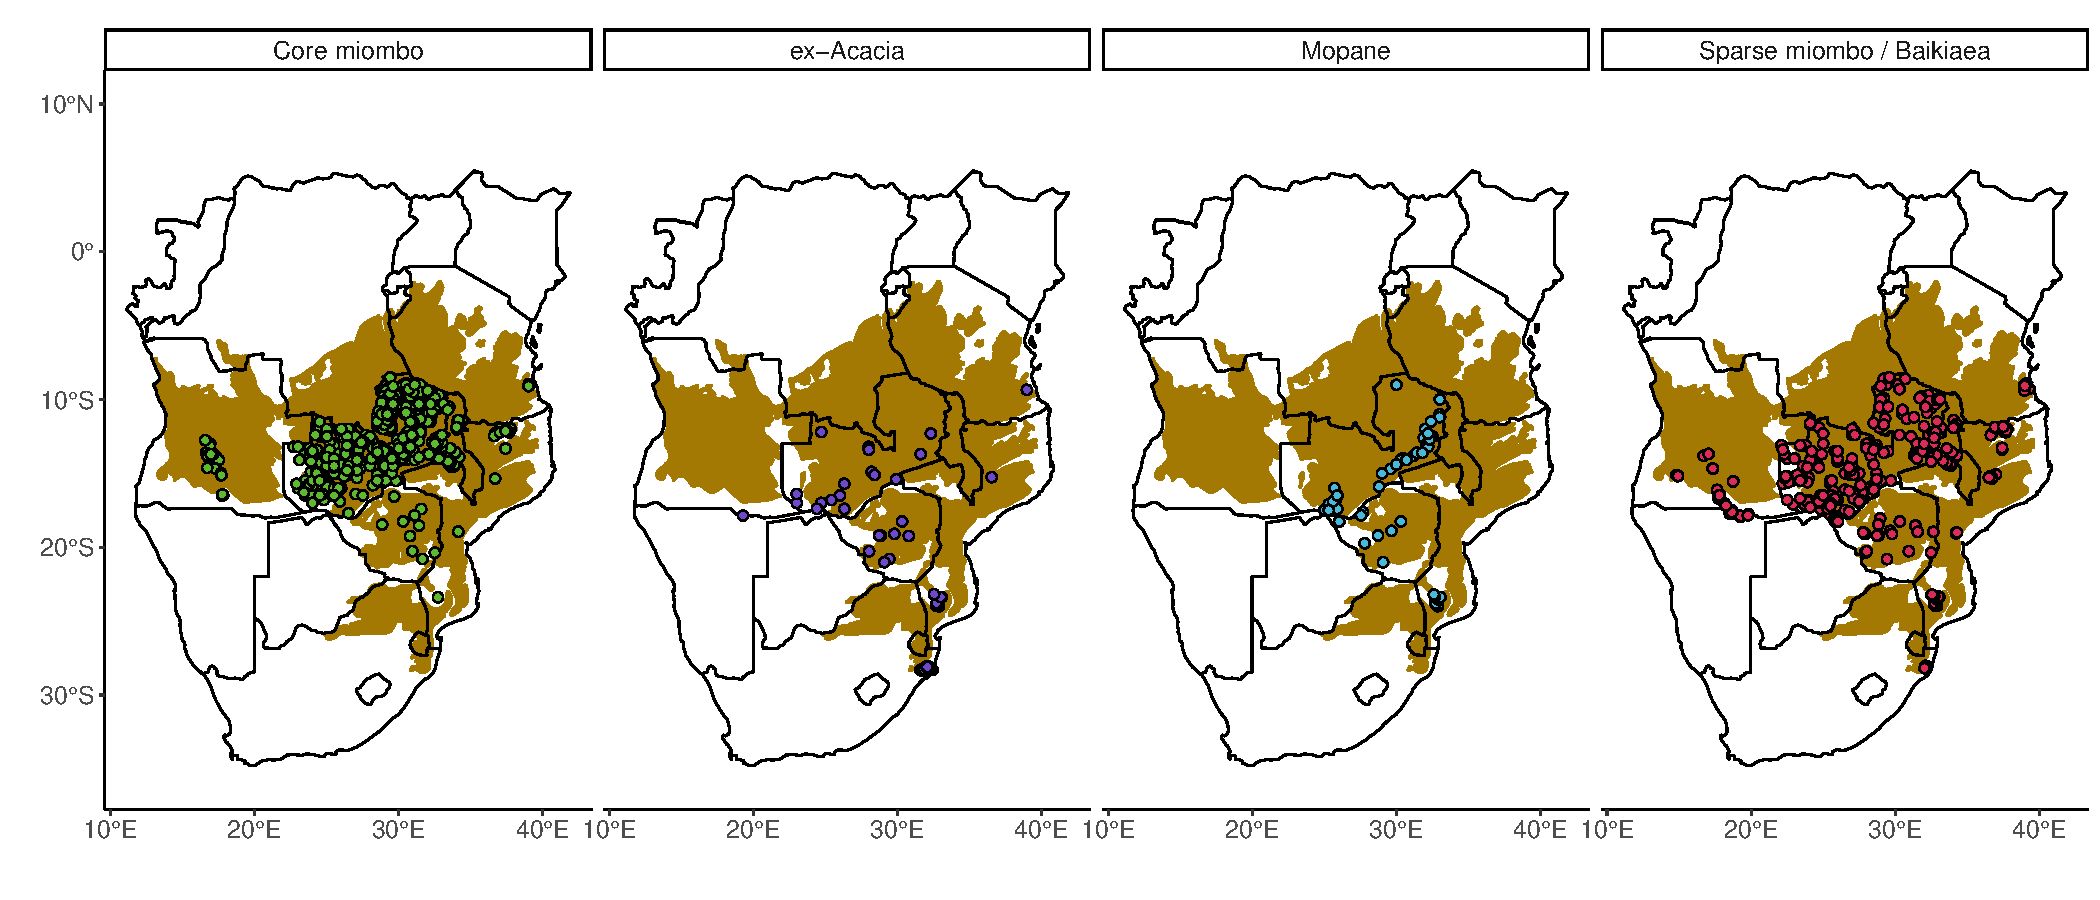
\includegraphics[width=\linewidth]{img/clust_map}
	\caption[Plot locations used in analysis, grouped by vegetation type]{The locations of the \nplots{} plots used in this study, with respect to the distribution of mesic savanna vegetation according to \citet{White1983}. Each panel shows plots categorised by their vegetation type as defined by the vegetation types in \autoref{befr:clust_summ}.}
	\label{befr:clust_map}
\end{figure}
\end{landscape}

\subsubsection{Structural equation modelling}
\label{befr:sssec:sem}

We used Structural Equation Modelling (SEM) to investigate the determinants of AGB. All SEMs were constructed and analysed in the `lavaan' package \citep{lavaan} in R version 4.1.0 \citep{R2020}. SEM was used because of its suitability for modelling complex causal interactions in ecological systems \citep{Lee2007}. A key aspect consideration in our decision to use SEM is that they can explicitly model and partition variance attributed to indirect effects, which is challenging in standard multiple regressions. Using SEMs also allowed us to describe latent variables such as `water availability', `soil fertility', and `disturbance' which have been suggested to act upon biodiversity and biomass/productivity in previous studies despite these factors not having directly observable measures in our dataset. SEM is also necessary to properly account for potential feedback mechanisms between aspects of environment and tree species diversity, which could otherwise increase the chances of Type I error and wrongly attribute inference due to the covariance of explanatory variables when using conventional regression analyses \citep{Nachtigall2003}.

We specified a conceptual model with factors expected to affect AGB: water availability, soil fertility, disturbance, tree species diversity, tree structural diversity and stem density (\autoref{befr:con_mod}). 

\begin{figure}
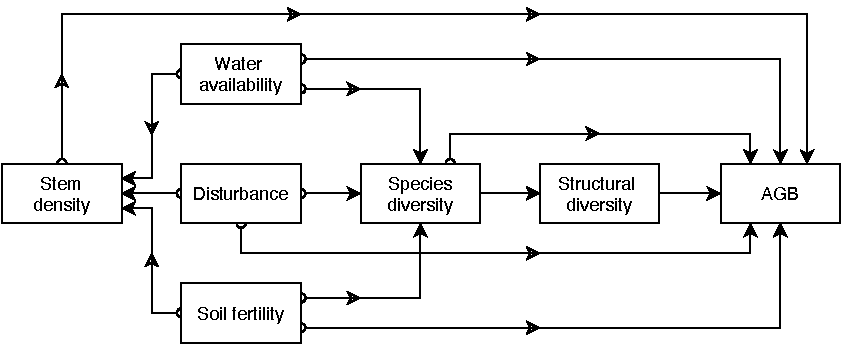
\includegraphics[width=\linewidth]{img/concept.drawio}
\caption[Conceptual model path diagram]{Conceptual Directed Acyclic Graph (DAG) showing the theoretical relationships between environmental factors, tree species diversity, tree structural diversity, stem density, and AGB (Above-Ground Woody Biomass). Hypothesised paths of causation are depicted as arrows from predictor to response. Open arrow heads track the direction of each arrow along its path.}
	\label{befr:con_mod}
\end{figure}

Observed variables were transformed to achieve normality where necessary and standardised to Z-scores prior to analysis (\autoref{befr:hist_raw}, \autoref{befr:hist_trans}). Standardisation allows path regression coefficients to be easily compared between paths in the same model to assess their relative effect size, and eliminates confusion in model interpretation arising from the observed variables being on different scales \citep{Beaujean2014}. Standardisation also controls for variables with variation across different orders of magnitude, which could otherwise prevent adequate model estimation from the covariance matrix in `lavaan'. To ensure that observed variables within a latent variable had consistent directions of influence, some observed variables had their sign reversed. For example, overall water availability is expected to decrease as soil sand content increases, therefore sand content was reversed for use in the water availability latent variable. Precipitation seasonality, and temperature stress were also reversed in this way to account for the direction of their effect on water availability. 

The factor loading of the observed variable assumed to contribute most to each latent variable were set to one, as per convention, with other observed variables being allowed to vary \citep{Beaujean2014}. We tested the robustness of our assumptions with a chi-squared test of all possible combinations of observed variable factor loadings set to one, while ensuring no factor loading were in excess of one. We found no significant difference between model specifications (p >0.05). Full Information Maximum Likelihood (FIML) was used in each model to estimate the values of missing data in each latent variable \citep{Cham2017}.

First, we used a simple mediation model which excluded the environmental covariates, to assess the role of tree species diversity and tree structural diversity in determining AGB. This model allowed direct effects of species diversity, structural diversity, and stem density on AGB, and also the indirect effect of species diversity on AGB via structural diversity. To explore variation in the model among woodland vegetation types, we fit the model both at the regional scale and for each vegetation type separately. We compared unstandardised path coefficients among the models for different vegetation types to understand the effect that vegetation type has on the relationship between tree species diversity, structural diversity, stem density and AGB. Path coefficients show the effect of a given path with other paths held constant. Models were estimated using the `MLM' estimator, because it is robust to multivariate non-normality \citep{Shapiro1983}. Model fit was evaluated using the robust Comparative Fit Index (CFI), the robust Tucker Lewis Index (TLI), the Root Mean Squared Error of Approximation (RMSEA) and the R\textsuperscript{2} coefficient of determination for AGB. We critically assessed model fit in each case, taking into consideration the recommendations of \citet{Hu1999} who define threshold values of acceptability for these model fit indices: CFI >0.85, TLI >0.85, RMSEA <0.15, alongside our judgement of the model estimates.

To explore the hypothesis that biodiversity effects on ecosystem function increase in strength as stem density increases, we repeatedly sub-sampled the available plot dataset to create \subn{} data subsets with similar stem density. For each data subset we separately fitted a model including tree species and structural diversity latent variables to predict AGB. As we controlled for stem density via the dataset sub-sampling process, the effect of stem density on AGB was not included in the model. We examined how the unstandardised path coefficients for each path in the SEM varied according to the median stem density of the data subsets. 

Second, we fitted the full model with environmental covariates, to understand the relative effects of water availability, soil fertility and disturbance on AGB, both directly and indirectly via species diversity and stem density. We compared standardised path coefficients among paths in the model to understand the relative contribution of each path to explain variance in AGB. Due to sample size issues, and because some vegetation types were narrow in their climate space, particularly in the water availability latent variable, we could not fit the model including environmental covariates separately for each vegetation type, as we encountered issues with model convergence. Preliminary models that included herbivore biomass from \citet{Hempson2017} did not converge. This is possibly due to the spatially coarse nature of the available data, or to collinearity with other variables, notably MAP and fire frequency. We therefore did not include herbivory in our final model.

\section{Results}
\label{befr:sec:results}

Pairwise correlations between all observed variables used in the Structural Equation Models (SEMs) showed that all tree species diversity (extrapolated tree species richness, Shannon equitability index) and structural diversity (coefficients of variation of DBH and height) variables had moderate positive correlations with AGB (\autoref{befr:corr_mat}, \autoref{befr:bivar_lm}). Stem density had the strongest correlation with AGB of all variables considered (\ccib{}). Environmental variables had weaker correlations with AGB than diversity variables, with all environmental variables having significant correlations with AGB, except fire frequency. The direction of these correlations was used as a test of our assumptions for the direction of influence of latent variables later used in the SEMs. MAP had positive correlations with all tree species diversity and structural diversity variables. Tree species diversity variables had clear positive correlations with stem density (species richness: \ccsi{}; Shannon equitability: \ccei{}), but structural diversity variables showed weak correlations with stem density (DBH CV: \ccdvi{}, Height CV: \cchvi{}).

\begin{figure}
	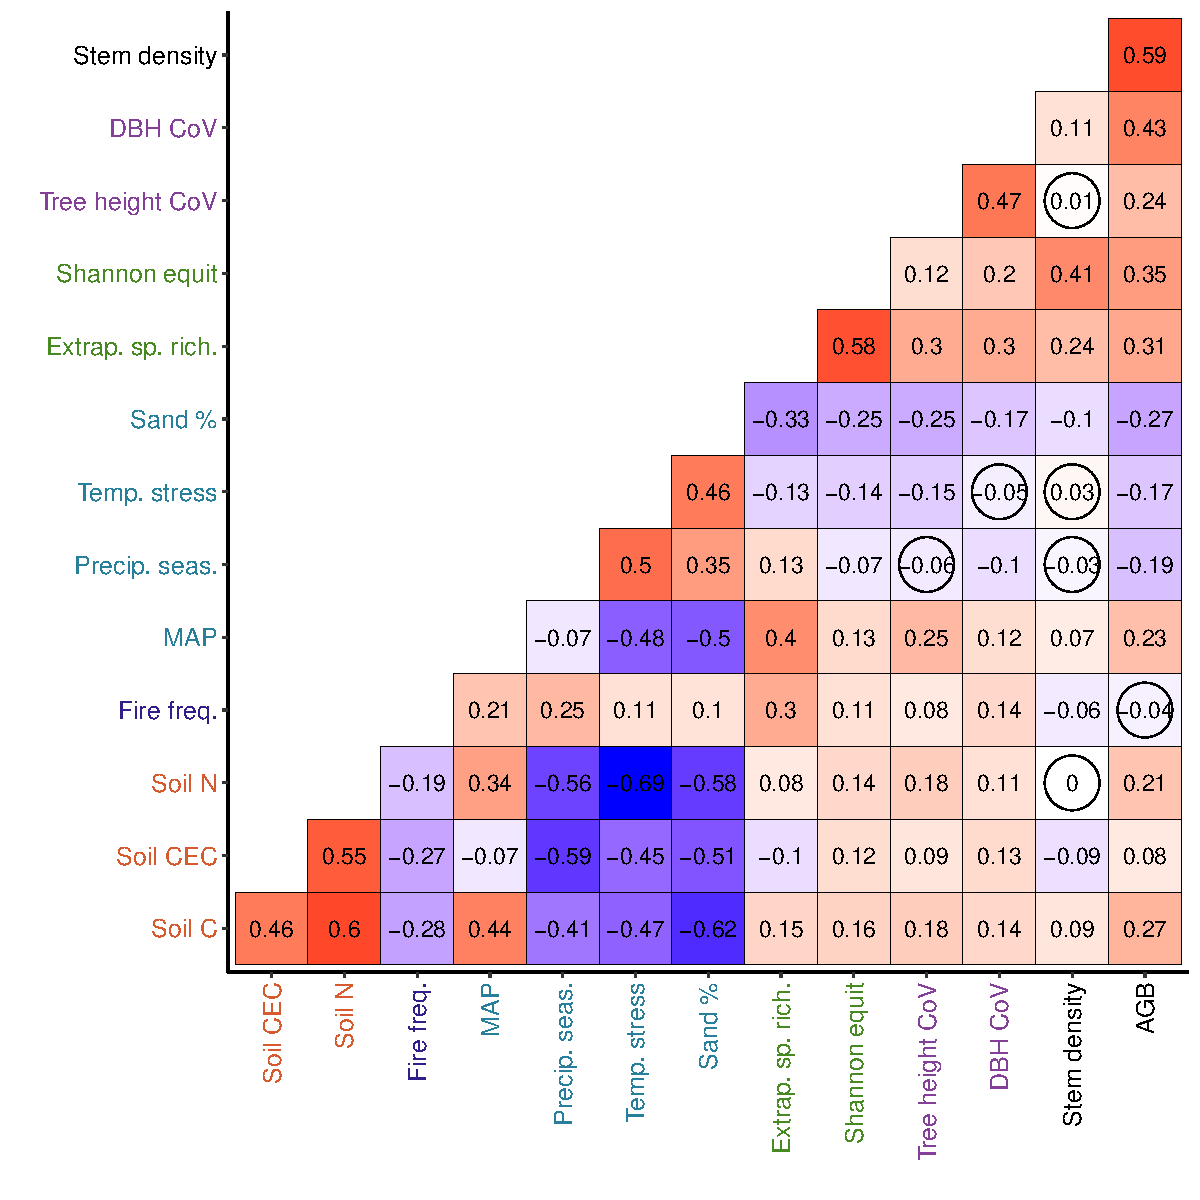
\includegraphics[width=\linewidth]{img/corr_mat}
	\caption[Correlation matrix of observed variables used in analysis]{Correlation matrix of standardised observed variables used in the SEMs (Structural Equation Models), with Pearson correlation coefficients ($r$) coloured according to sign ($+$ve red, $-$ve blue) and shaded by strength of correlation. Correlation coefficients marked by a circle indicate that the 95\% confidence interval of $r$ overlapped zero. Colours of variable names group them into latent variables used in the SEMs: red = soil fertility, blue = disturbance, turquoise = water availability, green = tree species diversity, purple = tree structural diversity. See \autoref{befr:corr_ci} for a full assessment of correlation fit statistics.}
	\label{befr:corr_mat}
\end{figure}

\subsection{Structural and species diversity models}
\label{befr:ssec:struc}

In the reduced SEM, which included stem density and the mediating effect of species diversity on AGB via structural diversity (\autoref{befr:struc_mod}), species diversity showed no direct effect on AGB (\strucbetadb{}), but did have an indirect positive effect via structural diversity (\strucbetadib{}) (\autoref{befr:struc_mod}). Model fit was good with high factor loading for all observed variables. All other path coefficients were significant (p <0.01) (\autoref{befr:struc_model_fit_clust_stats}). The R\textsuperscript{2} of AGB was \strucrsq{}. The strongest direct effect on AGB was from stem density (\strucbetaib{}).

\begin{table}
	\caption[Model fit statistics per vegetation type]{Model fit statistics for Structural Equation Models investigating the effects of tree diversity and stem density on AGB (\autoref{befr:struc_mod}). N = number of plots in cluster, $\chi^{2}$ = Chi-squared fit statistic, DoF = model degrees of freedom, CFI = Comparative Fit Index, TLI = Tucker-Lewis Index, RMSEA = Root Mean Square Error of Approximation, R\textsuperscript{2} AGB = model R\textsuperscript{2} for AGB (Above-Ground Biomass).} 
	\label{befr:struc_model_fit_clust_stats} 
	\begin{tabular}{lS[table-format=4.0]S[table-format=2.2]S[table-format=1.0]S[table-format=1.3]S[table-format=1.3]S[table-format=1.3]S[table-format=1.3]} 
\toprule
{Cluster} & {N} & {$\chi$\textsuperscript{2}} & {DoF} & {CFI} & {TLI} & {RMSEA} & {R\textsuperscript{2} AGB} \\
\midrule
Core miombo & 523 & 78.67 & 6 & 0.904 & 0.759 & 0.14 & 0.49 \\ 
ex-Acacia & 188 & 9.57 & 6 & 0.952 & 0.879 & 0.13 & 0.83 \\ 
Mopane & 58 & 19.88 & 6 & 0.834 & 0.584 & 0.24 & 0.51 \\ 
Baikiaea & 466 & 43.87 & 6 & 0.914 & 0.784 & 0.13 & 0.58 \\ 
All & 1235 & 91.38 & 6 & 0.937 & 0.843 & 0.12 & 0.49 \\ 
\bottomrule
\end{tabular} 
\end{table} 


\begin{figure}
	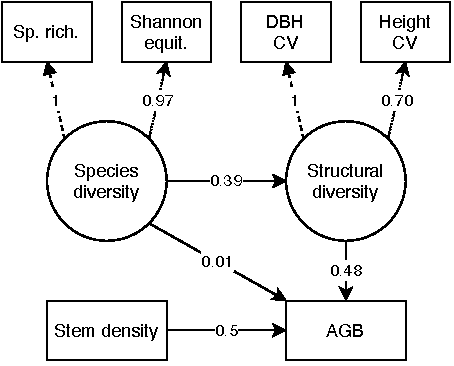
\includegraphics[width=0.5\linewidth]{img/struc.drawio}
	\caption[Path diagram for vegetation type model]{Path diagram with regression coefficients for the tree diversity SEM (Structural Equation Model), including plots from all vegetation clusters. Latent variables are shown as circles while observed variables are shown as rectangles. Standardised path coefficients are shown as solid arrows pointing from predictor to response with the effect size of the path coefficient expressed in terms of standard deviations on the latent variable response scale. The observed variables that inform the latent variables are connected by dotted arrows, and observed variables with loading set to one are connected by dashed arrows. Measurement errors of exogenous variables are omitted for clarity.}
	\label{befr:struc_mod}
\end{figure}

\subsection{Variation among vegetation types}
\label{befr:ssec:veg}

When the tree species and structural diversity model (\autoref{befr:struc_mod}) was refitted separately using data from each of the four vegetation types, we found that the effect sizes of each latent variable remained largely similar, though model fit varied. The direct effect of tree species diversity on AGB was positive and marginally significant in ex-Acacia (\strucbetacsb{}) but negligible in Mopane (\strucbetadsb{}), Baikiaea (\strucbetaasb{}) and Core miombo (\strucbetabsb{}) (\autoref{befr:struc_model_slopes_all}). Relationships among structural diversity and AGB remained generally similar, with the same sign and overlap between the 95\% confidence intervals of path coefficients. The R\textsuperscript{2} of AGB was highest in ex-Acacia shrubland (R\textsuperscript{2} = \struccrsq{}) and lowest in Baikiaea (R\textsuperscript{2} = \strucarsq{}). The total effect of species diversity on AGB remained strongly positive and there was a positive direct effect of species diversity on structural diversity, across all vegetation types. All models had adequate goodness-of-fit (\autoref{befr:struc_model_fit_clust_stats}), though confidence intervals around the unstandardised path coefficients were wide particularly for Mopane and ex-Acacia. $\chi^{2}$ statistics were high for some vegetation types, but this appears to be highly correlated with sample size for each vegetation type \citep{Hooper2008}.

\begin{figure}
	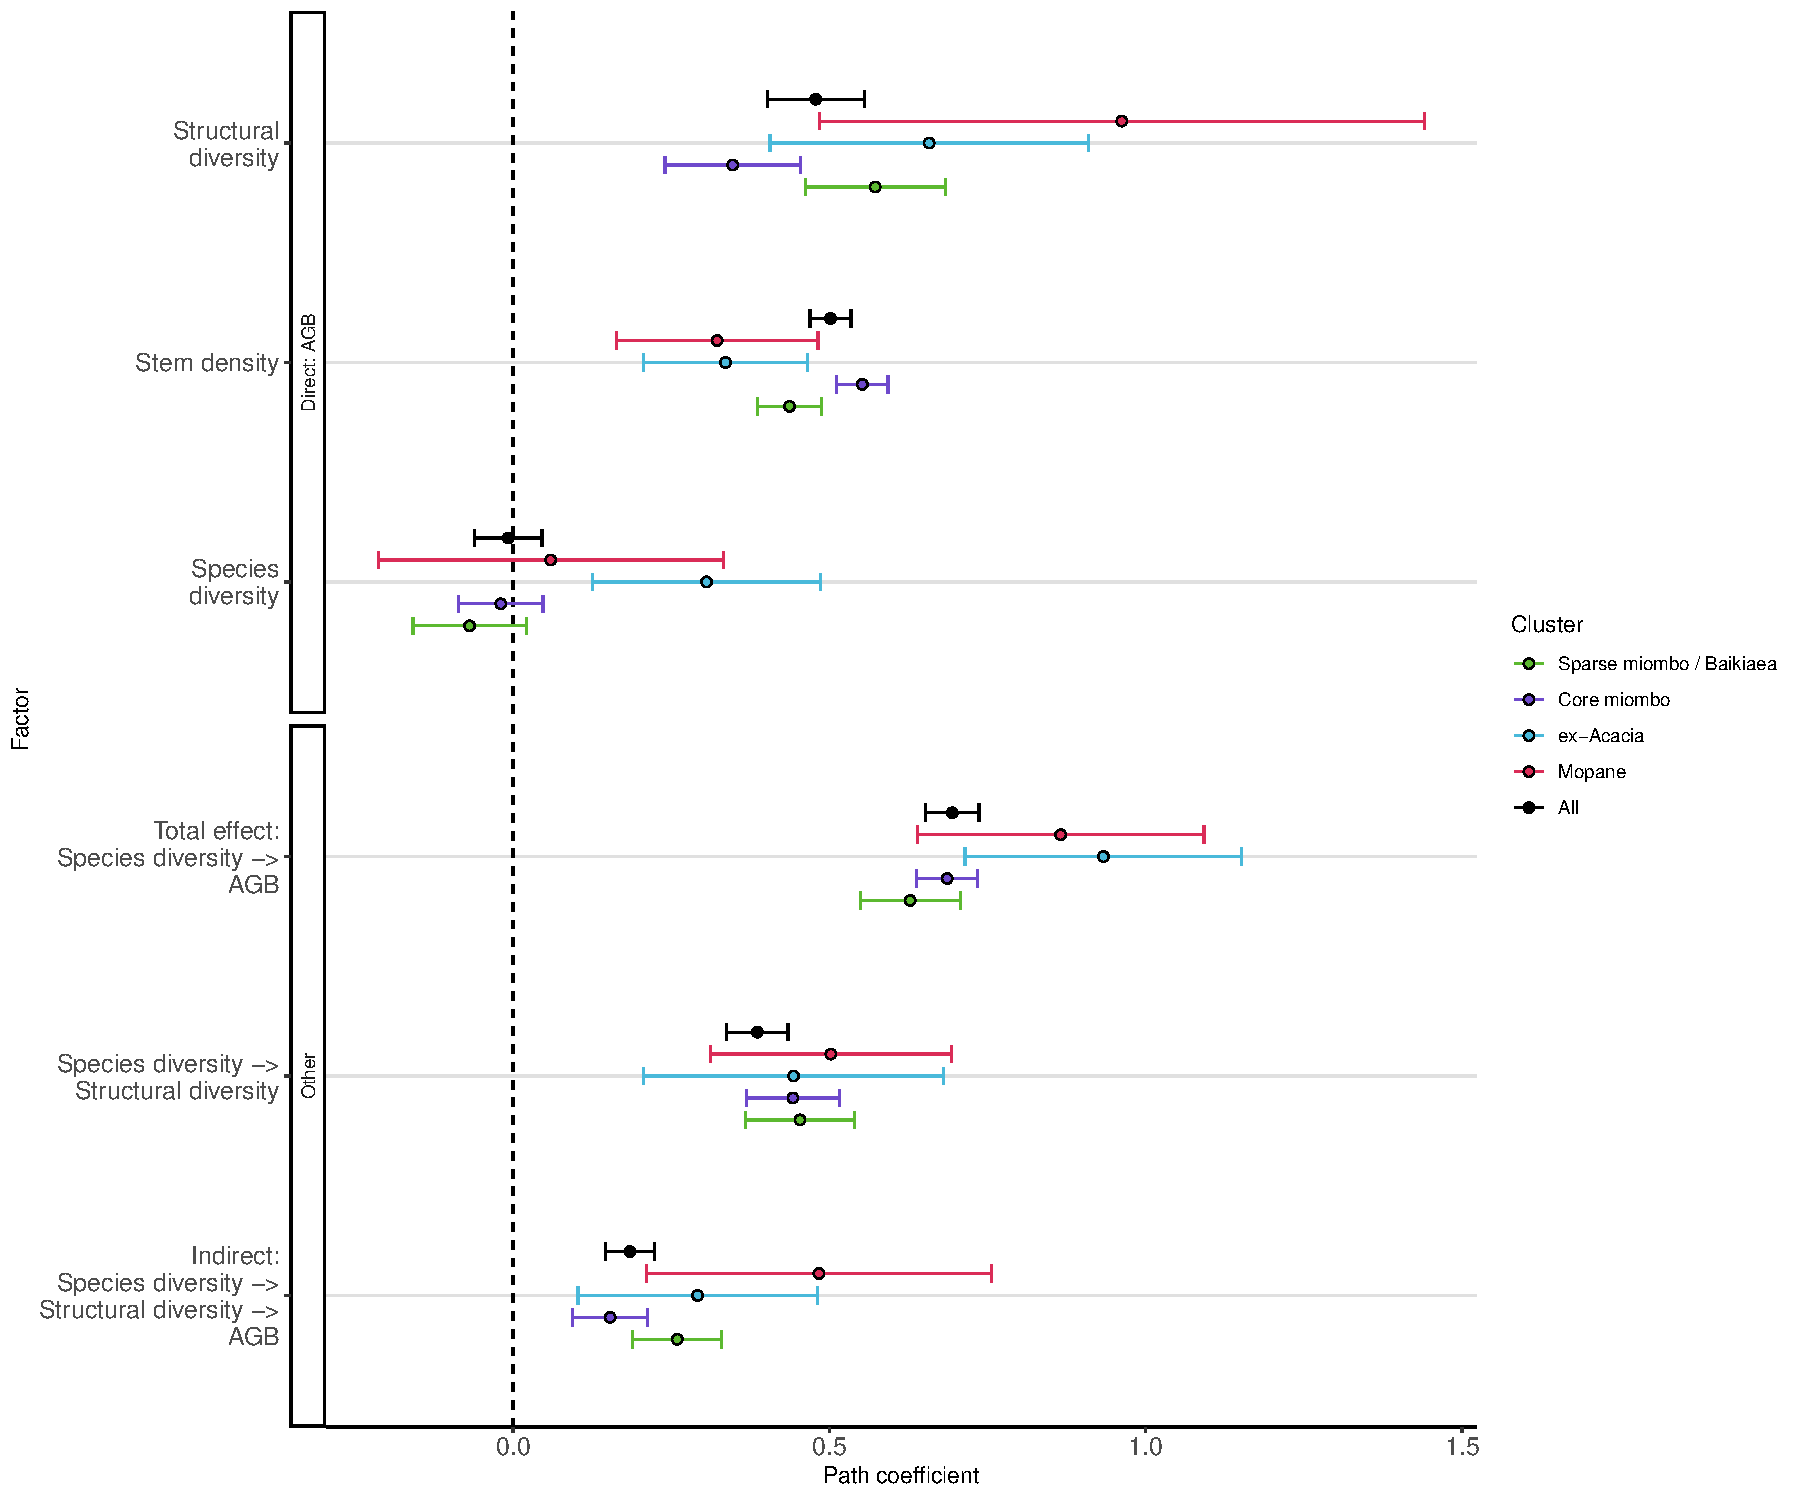
\includegraphics[width=\linewidth]{img/struc_model_slopes_all}
	\caption[Path coefficients for vegetation type model]{Unstandardised path coefficients for the effects of tree diversity on AGB (Above-Ground Woody Biomass), mediated by the effect of stand structural diversity. Path coefficients are $\pm$1 standard error. Path coefficients where the interval (standard error) does not overlap zero are considered to be significant effects.}
	\label{befr:struc_model_slopes_all}
\end{figure}

\subsection{Moderation of diversity effect by stem density}
\label{befr:ssec:stems}

In the sub-sampling of the plot dataset by stem density, we found an increasing positive effect of tree species diversity on AGB as stem density increased (\autoref{befr:sem_struc_stems_ha}e). There appears to be a minimum stem density threshold at c. 180 stems >10 cm DBH ha\textsuperscript{-1} below which there appears to be a reasonably constant baseline effect of tree diversity on biomass (\autoref{befr:sem_struc_stems_ha}b). The effect of structural diversity on AGB appears to remain constant with increasing stem density (\autoref{befr:sem_struc_stems_ha}d). The indirect effect of tree species diversity on AGB via structural diversity increases as stem density increases (\autoref{befr:sem_struc_stems_ha}c). 

\begin{figure}
	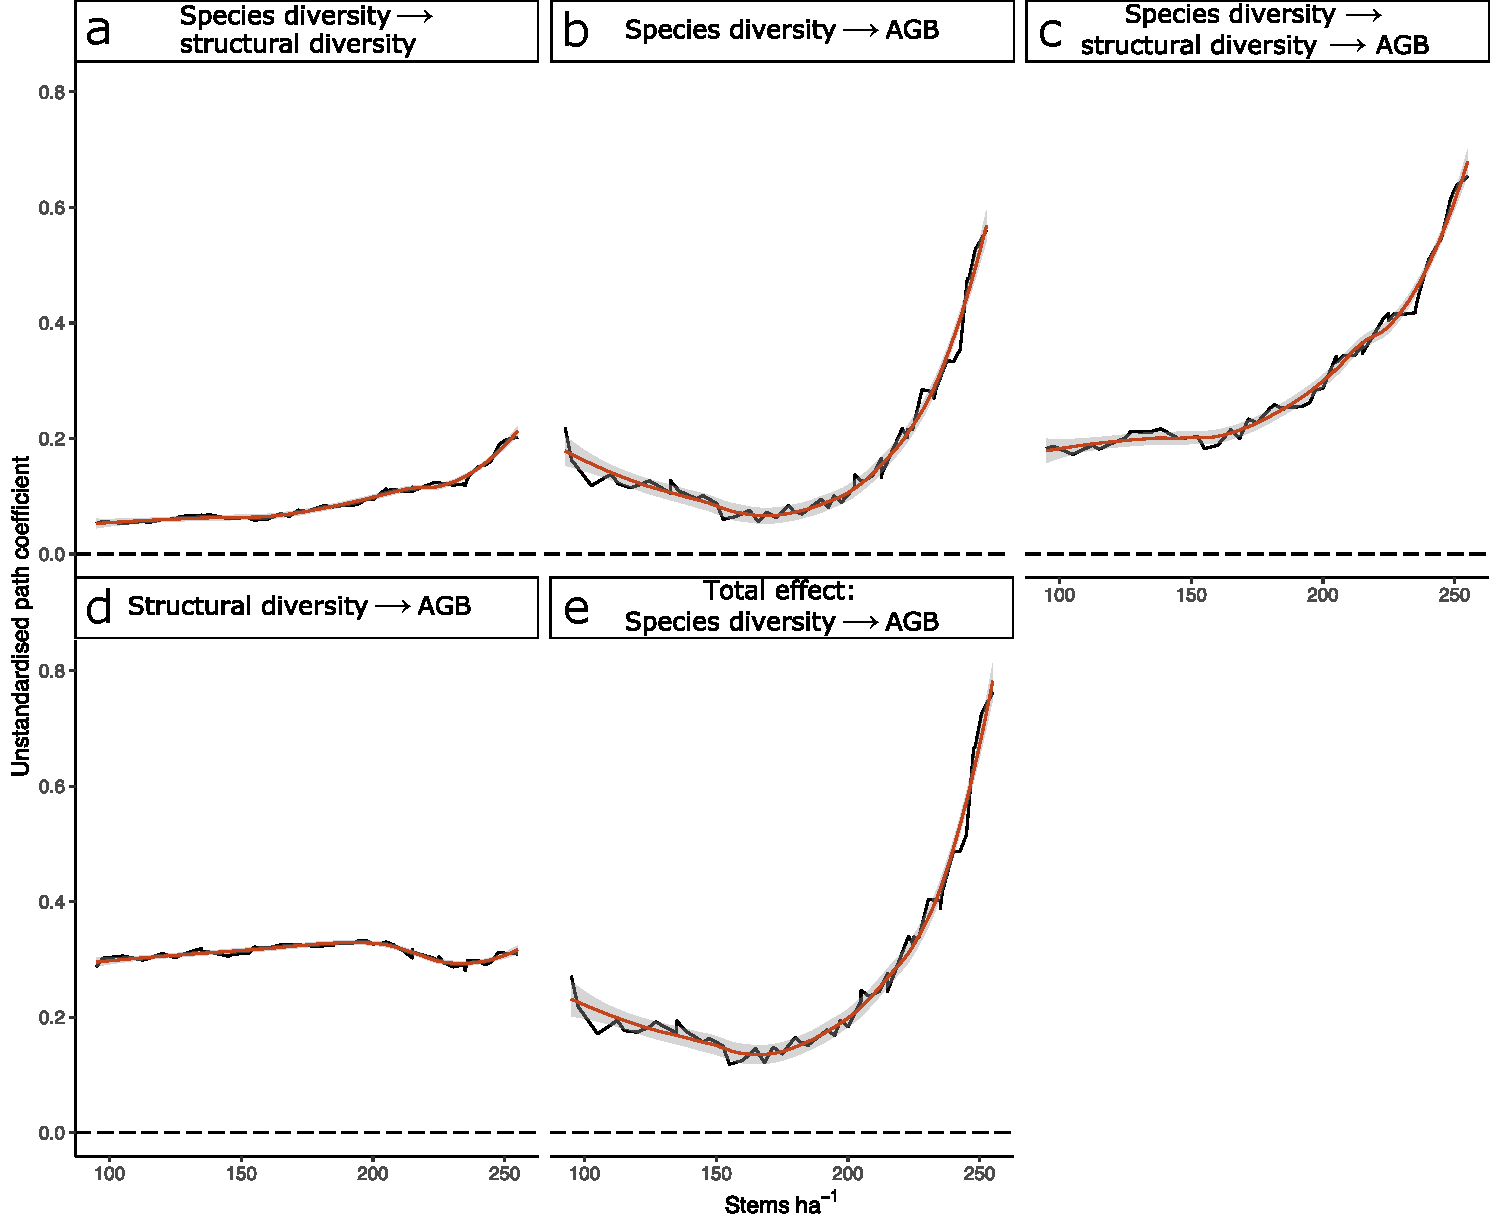
\includegraphics[width=0.8\linewidth]{img/sem_struc_stems_ha}
	\caption[Effect of stems density on path coefficients]{Line plots showing the variation in SEM (Structural Equation Model) path coefficients among latent variables, across datasets with different mean stem density. Smoothed lines are loess curves with $\pm1$ standard error shaded bars. AGB = Above-Ground woody Biomass. Arrows in plot titles indicate causal paths in SEM models. Where multiple arrows are present, as in c), this indicates an indirect pathway via an intermediate variable. a) shows the direct effect of species diversity on structural diversity. b) and d) show the direct effects of species diversity and structural diversity on AGB, respectively. c) shows the indirect effect of species diversity on AGB via structural diversity. e) shows the total effect of species diversity on AGB, incorporating both the direct effect and the indirect effect via structural diversity.}
	\label{befr:sem_struc_stems_ha}
\end{figure}

\subsection{Environmental covariates and tree diversity}
\label{befr:ssec:env}

A model incorporating the latent variables of water availability, soil fertility and disturbance by fire showed that the total effect of tree species diversity on biomass was similar to that of water availability, soil fertility and disturbance (\autoref{befr:full_mod}, \autoref{befr:full_model_slopes}). The direct effects of water availability, soil fertility and disturbance on AGB were negligible (water: \fmbetamb{}, soil: \fmbetasb{}, disturbance: \fmbetafb{}), with nearly all of their observed effects on AGB coming from the indirect paths via stem density (water: \fmbetamib{}, soil: \fmbetasib{}, disturbance: \fmbetafib{}) and species diversity (water: \fmbetamd{}, soil: \fmbetasd{}, disturbance: \fmbetafd{}). MAP and soil sand content had the greatest contributions to the latent variable of water availability. Model fit was acceptable: CFI = 0.925, TLI = 0.900, and RMSEA = \fmrmsea{}, R\textsuperscript{2} of AGB = \fmrsq{}. 

Similar to the model that only considered tree species and structural diversity (\autoref{befr:struc_mod}), the direct effect of species diversity on structural diversity was positive, while structural diversity itself had a positive effect on AGB, leading to a strong positive indirect effect of species diversity on AGB via structural diversity (\fmbetadhb{}) when environmental covariates were accounted for. Again, the direct effect of species diversity on AGB was negligible (\fmbetadb{}). The total effect of species diversity on AGB was positive (\fmbetatotaldb{}). Compared to the simple model with no environmental covariates, the total explanatory power of tree species diversity and structural diversity in this model decreased, but the predictive power of the model as a whole increased.

\begin{figure}
	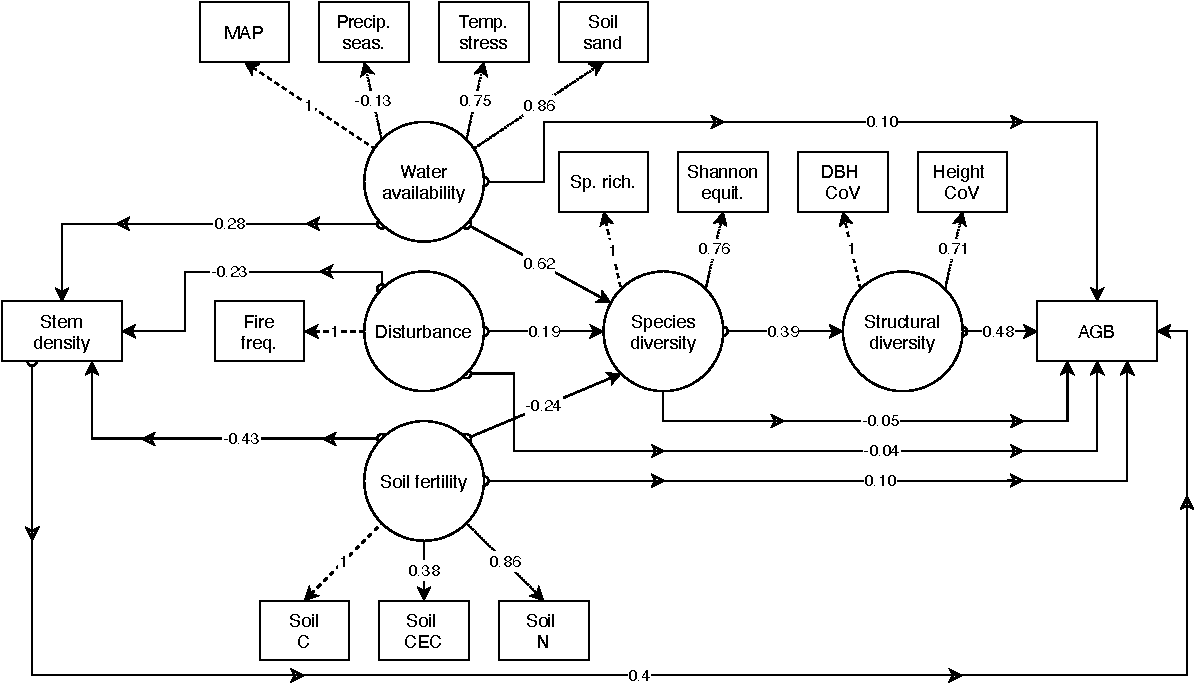
\includegraphics[width=\linewidth]{img/full.drawio}
	\caption[Path diagram of full Structural Equation Model]{Path diagram with regression coefficients for the SEM (Structural Equation Model) incorporating environmental covariates and tree species and structural diversity across all five vegetation types. Latent variables are shown as circles while observed variables are shown as rectangles. Standardised path coefficients are shown as solid arrows pointing from predictor to response, with the effect size of the path coefficient expressed in terms of standard deviations on the latent variable response scale. Observed variables that inform the latent variables are connected by dotted arrows, observed variables with loading set to one are connected by dashed arrows. Measurement errors of exogenous variables are omitted for clarity.}
	\label{befr:full_mod}
\end{figure}

\section{Discussion}
\label{befr:sec:discussion}

We assessed the importance of a) tree species diversity, b) tree structural diversity, c) resource availability, d) disturbance by fire, e) organismal density and their interactions on above-ground woody biomass (AGB) across southern African savannas and woodlands, using a network of \nplots{} woodland plots in conjunction with Structural Equation Modelling (SEM). We found support for a general positive relationship between tree species diversity and AGB, operating indirectly via structural diversity (H\textsubscript{1}). Tree species diversity, structural diversity and stem density accounted for \smrsq{}\% of the variation in AGB across the region, while models for specific vegetation types showed even greater explanatory power in some cases (\autoref{befr:struc_model_fit_clust_stats}). Within the latent variable of tree species diversity we found similarly strong factor loading for both species richness and abundance evenness. This demonstrates that species richness and abundance evenness measure different and largely uncorrelated axes of diversity. We found that the effect of tree species diversity on AGB increased with stem density (H\textsubscript{2}), with an apparent threshold of 180 stems >10 cm DBH ha\textsuperscript{-1}, below which the effect of species diversity on AGB remained at a low baseline level. The strongest direct effect on AGB was that of stem density. When the effects of water availability, soil fertility and disturbance by fire were controlled for, the total explanatory power of tree species diversity and structural diversity decreased, but the predictive power of the model increased, suggesting that it is important to control for environmental covariates to understand the true effect of tree species diversity on AGB in regional scale assessments of the BEFR.

\subsection{Inter-related effects of tree species and structural diversity on AGB}
\label{befr:ssec:struc_agb}

We found a consistent positive effect of tree species diversity on AGB. Within southern African woodlands we therefore find support for the hypothesis that higher tree species richness and evenness leads to higher above-ground woody biomass. This finding is in agreement with many other studies across different ecosystems and biomes, supporting the idea that there is a generalisable positive association between biodiversity and ecosystem function \citep{Liang2016, Cardinale2009}. Our study provides a novel dissection of the mechanisms underlying this relationship, particularly in the context of southern African woodlands, a disturbance-driven and poorly studied ecological system.

Much of the total variation in AGB was driven by variation in organismal density. It is possible that within southern African woodlands a higher species diversity allows for a higher stem density through niche separation, which reduces competition between species occupying varying niche space, leading to an increase in total AGB per unit area. The opposite causation is also plausible however, with increased stem density causing higher species richness through an increased probability of encountering new species. We attempted to correct for the correlation between species richness and stem density using extrapolated species richness, which extrapolates a rarefaction curve to its predicted asymptote, thus estimating the total landscape level species richness which is independent of plot size and stem density. We suggest therefore that an increase in tree species diversity through species richness and evenness produces an assemblage of species which can utilise more available light and moisture, resulting in greater plot level AGB. This is supported by the moderately strong indirect positive effect of tree species diversity on AGB via structural diversity, and the positive effect of water availability on AGB via stem density in the model which included environmental covariates. 

We found evidence that tree species diversity led to an increase in AGB indirectly via tree structural diversity, and we therefore find support for our second hypothesis H\textsubscript{2}. A higher tree species diversity allows for a greater structural diversity of trees, i.e. greater variation in DBH and height. This may act as a mechanism for niche complementarity, with a canopy of diversely-sized trees able to take advantage of a greater proportion of the available light. Additionally, the volume of tree above-ground structures is generally correlated with the volume of below-ground structures \citep{Paul2019}. In water and nutrient limited ecosystems especially, variation in rooting depth may constitute a second related axis of niche partitioning driving the observed positive effect of above-ground structural diversity on AGB \citep{Kulmatiski2013}. Although we did not measure them here, we would also expect that tree species diversity allows for a greater range of tree functional forms \citep{Pretzsch2014}, i.e. wider variation in canopy shape and overall growth form; broad flat crowns vs. narrow deep crowns, for example. In forests, where the tree canopy is effectively closed, as the stand matures a more diverse canopy emerges via competition and tree mortality events which open canopy gaps \citep{Muscolo2014}. Indeed, our finding that the strength of the effect of tree diversity on AGB increases with stem density supports this mechanism (\autoref{befr:sem_struc_stems_ha}). At low stem densities, competition between mature trees may not occur, meaning that the niche complementarity effect provided by an increase in tree species richness may not be present, accounting for the small effect of tree species diversity on AGB below c. 180 trees ha\textsuperscript{-1}. In frequently disturbed woodlands such as those studied here, a woodland canopy similar to that of a forest is frequently not reached. Instead, a simple open canopy is maintained that can be made more complex and productive via an increase in species diversity.

Alternatively, due to the non-linear relationship between biomass and tree size \citep{Bastin2018}, the positive relationship between structural diversity and biomass may also be partly driven by an increased number of large sized trees in plots with higher structural diversity, with large trees contributing disproportionately to biomass. The positive effect of species diversity on AGB via structural diversity may therefore be due to selection effects, with higher diversity plots supporting larger trees due to species specific variation in functional form \citep{Diaz2015}.

\subsection{Organismal density and disturbance}
\label{befr:ssec:disturbance}

Disturbance by fire had a negative total effect on AGB, with most of this negative effect coming from the indirect pathway via stem density. This is expected as increased fire frequency is a key mechanism by which savannas maintain an open canopy, rather than shifting to a closed canopy forest \citep{Staver2011}. Previous studies have found that southern African woodlands with higher species diversity tend to experience less frequent disturbance by fire and tend to form a more closed canopy with a sparse understorey \citep{Chidumayo2013, Mutowo2012}. In our study however, we found a positive effect of fire frequency on species diversity, perhaps suggesting that disturbance prevents domination of woodlands by a single dominant species \citep{Chidumayo2013, Durigan2020, Staver2009}. It is suggested that in savannas where the tree-species pool is largely adapted to fire, increased fire may actually increase tree species diversity by allowing weak competitors to co-exist. 

Disturbances such as fire have the potential to reduce both species diversity and above-ground biomass in the short term, due to increased mortality \citep{Huston2014}. Unless this effect is accounted for, there is the potential for mistaken causality as both diversity and biomass may correlate. In our model, time since disturbance is accounted for within each plot via the stem density term. Disturbance reduces stem density of large stems (>10 cm DBH), which is expected to increase until the effects of competition preclude further increase \citep{Johnson2012}. Furthermore, our rarefied measure of species diversity accounts for variation in sampling effort and is therefore independent of stem density. Tree species richness should also increase with time since disturbance as with increased stem density the likelihood of including a new species also increases. Outside of the stem density effect, there are multiple causes for variation in tree species diversity in this study. Vegetation types and localities differ in their available species pool, for example. Variation in abiotic environmental factors will also affect species accumulation. 

\subsection{Effects of water availability and soil fertility}
\label{befr:ssec:water}

Water availability had a positive total effect on AGB, comparable in size to the total effect of tree species diversity on AGB, while soil fertility had a negative total effect. We expected that higher water availability and soil fertility would lead to higher AGB under the assumption that higher resource availability would allow for a greater stem density per unit area, greater productivity per unit area and additionally greater tree species diversity due to niche partitioning \citep{Kraaij2006, Shirima2015b}. Previous studies in tropical forests have shown that water availability increases AGB both directly and indirectly via increasing tree species diversity and via increasing stand structural diversity \citep{Ali2019a, Ali2019b, Poorter2017}. In this study, we observed indirect positive effects of water availability on AGB via species diversity and a positive but only marginally significant direct effect on AGB. Compared to moist tropical forests, water availability is more of a limiting factor to tree growth in southern African woodlands, which experience frequent drought. 

A negative total effect of soil fertility on AGB is in contrast to other studies in the region and general ecological theory, which predicts a positive effect of soil nutrients on biomass \citep{Scarascia2000}. The negative total effect of soil fertility on AGB was driven mostly by an indirect negative effect via stem density. The direct effect on AGB however, remained positive and marginally significant, as expected. Model estimates of the effect of soil on AGB were poorly constrained compared with other latent variables. This wide standard error on the model predictions is possibly due to the coarseness and nature of the soil data we used. SoilGrids provides modelled data at 250 m resolution, while soil structure and nutrient content varies at much finer scales in southern African woodlands \citep{Muledi2017, Bucini2007}. It is therefore not surprising that this model path is poorly constrained. \citet{Lehmann2014} found similarly weak and poorly constrained relationships for soil in a Structural Equation Model including precipitation, temperature, soil, and fire to predict tree basal area in southern African woodlands. Plot-specific soil data are time-consuming to collect and difficult to compare across studies when different protocols are used. Our study points to the need for further effort in this regard, which may reveal interesting findings about the complex interactions between soil, disturbance and tree diversity in southern African woodlands. Alternatively, \citet{Gourlet2011} found that environmental filtering of fast-growing species with low wood density on resource poor soils resulted in a decoupling of the soil fertility - AGB relationship. It is possible that at regional scales, variation in species composition could offset resource availability constraints on AGB. However, unlike \citet{Gourlet2011} disturbance by fire in our study region may further complicate this environmental filtering effect.

\subsection{Vegetation type responses}
\label{befr:ssec:veg_type_response}

All four vegetation types produced similar results in the simple SEM, with a positive total effect of species diversity on AGB, the majority being indirectly via structural diversity. This demonstrates the robustness of our results, showing they are generalisable across vegetation types in southern Africa. It also demonstrates that similar ecosystem processes are occurring in these vegetation types, despite variation in species composition, overall species richness and mean biomass.

Core miombo and Baikiaea woodland vegetation exhibited a small negative direct effect of tree species diversity on AGB, while the total effect, incorporating the indirect effect via structural diversity, remained positive in these vegetation types. Compared to ex-Acacia and Mopane woodlands, miombo woodlands have higher median tree species richness. Ex-Acacia and Mopane woodlands are dominated by fewer tree species, notably \textit{Senegalia} spp. in ex-Acacia woodlands and \textit{Colophospermum mopane} in Mopane woodlands, which can produce large canopy dominating trees in the so-called ``Cathedral mopane''. We postulate that the slight negative effect of tree species richness on AGB in miombo woodlands may be due to an increase in interspecific competition through canopy crowding, but that this effect is not present in ex-Acacia and Mopane woodlands, where the top level of the woodland canopy is dominated often by a single species. 

Higher functional redundancy among tree species in miombo woodlands may lead to smaller trees with lower AGB in the most diverse plots, more resembling thicket vegetation and suppressing the few species which tend to create high biomass, such as \textit{Julbernadia} and \textit{Brachystegia} spp.. In the species-poor Mopane and ex-Acacia woodlands however, the addition of extra species may fill a greater proportional niche space, thus increasing total AGB more. 

Despite Mopane woodland having very low species diversity generally, with often monospecific stands \citep{Timberlake2010}, a positive effect of tree species diversity on AGB was observed. In previous studies across multiple biomes it has been found that the effect of adding species on ecosystem function is stronger in low diversity assemblages \citep{Cardinale2006, Srivastava2005}. This has been attributed to an increase in functional redundancy as species diversity increases. Mopane woodlands also have a negligible effect of species diversity on structural diversity. This may be due to the particular functional forms of species which co-exist with \textit{C. mopane}, many of which are small shrub-like trees rather than large canopy trees \citep{Timberlake2010}. Larger canopy trees tend to have greater variation in physical structure \citep{Seidel2019}, which would drive an effect of species diversity on structural diversity as we observed in miombo woodlands.

Ex-Acacia woodlands showed the strongest total effect of species diversity on AGB and was the only vegetation type to show a significant positive direct effect of species diversity on AGB. Ex-Acacia woodlands also had relatively low median species richness compared to miombo, but the addition of new species appears to make a larger difference to the AGB of these plots than in Mopane woodlands. We suggest that this is due mostly to the particular identity of species found in ex-Acacia woodlands and their contribution to ecosystem functioning. Unlike Mopane woodlands, ex-Acacia woodlands contain a wider variety of species which can grow to large canopy trees, albeit at low densities, especially in transition zones with miombo woodlands. Additionally, many more species species in ex-Acacia woodlands are found in the Mimosoideae and Papilionoideae sub-families, of which most are nitrogen-fixing \citep{Tedersoo2018}. Nitrogen availability is often a limiting factor in productivity, making nitrogen-fixing species strong competitors. It is possible that in ex-Acacia dominated woodlands, the presence of a large number of nitrogen-fixing tree species reduces functional redundancy, meaning that the effect of adding species on ecosystem function saturates at a higher species richness.

\section{Conclusion}
\label{befr:sec:conclusion}

In this study we found that even in highly disturbed southern African woodlands, there exists a generalisable positive association between tree species diversity and ecosystem function, quantified as above-ground woody biomass (AGB). Our findings contribute to our understanding of a universal biodiversity-ecosystem function relationship, one which is moderated in a predictable manner by environmental covariates and their interaction with biodiversity and ecosystem structure. We found that the multiple vegetation types which comprise southern African woodlands exhibit similarities in the relationship between species diversity and woody biomass, suggesting that similar processes operate across the region to determine ecosystem function. We advocate for explicit inclusion of environmental covariates in regional scale models of biodiversity and ecosystem function. We assert that this is necessary to develop our understanding of the biodiversity-ecosystem function relationship in real-world ecosystems, to progress from experimental mesocosms. We found that much of the effect of species diversity on biomass exists as an indirect effect by increasing the structural diversity of trees, exemplifying a key mechanism by which tree species diversity determines ecosystem function in savannas, woodlands and forests, where trees comprise a significant, canopy-forming component. The presence of a stem density threshold above which the effect of tree species diversity on AGB increases clearly implies the presence of niche complementarity effects in southern African woodlands, an aspect which has often been overlooked in previous studies despite its intuitive logic as a determinant of niche complementarity effects in wooded ecosystems. Our study shows that biodiversity change through extensive human-induced land use change in this region will have the greatest negative impact on ecosystem function in areas of high stems density, and in certain vegetation types, specifically Mopane and ex-Acacia woodlands. This raises concerns about the robustness of these ecosystems to further resource extraction and biodiversity loss. Finally, our results provide further evidence of the complex interaction of factors governing biomass and therefore carbon dynamics in disturbance-driven wooded ecosystems, which currently represent the greatest uncertainty in the global terrestrial carbon sink.

\newpage{}
\FloatBarrier{}
\begingroup
\setstretch{1.0}
\printbibliography[heading=subbibintoc]
\endgroup

\section{Supplementary material}
\label{befr:sec:supp}

\begin{supplement}

\begin{figure}[H]
	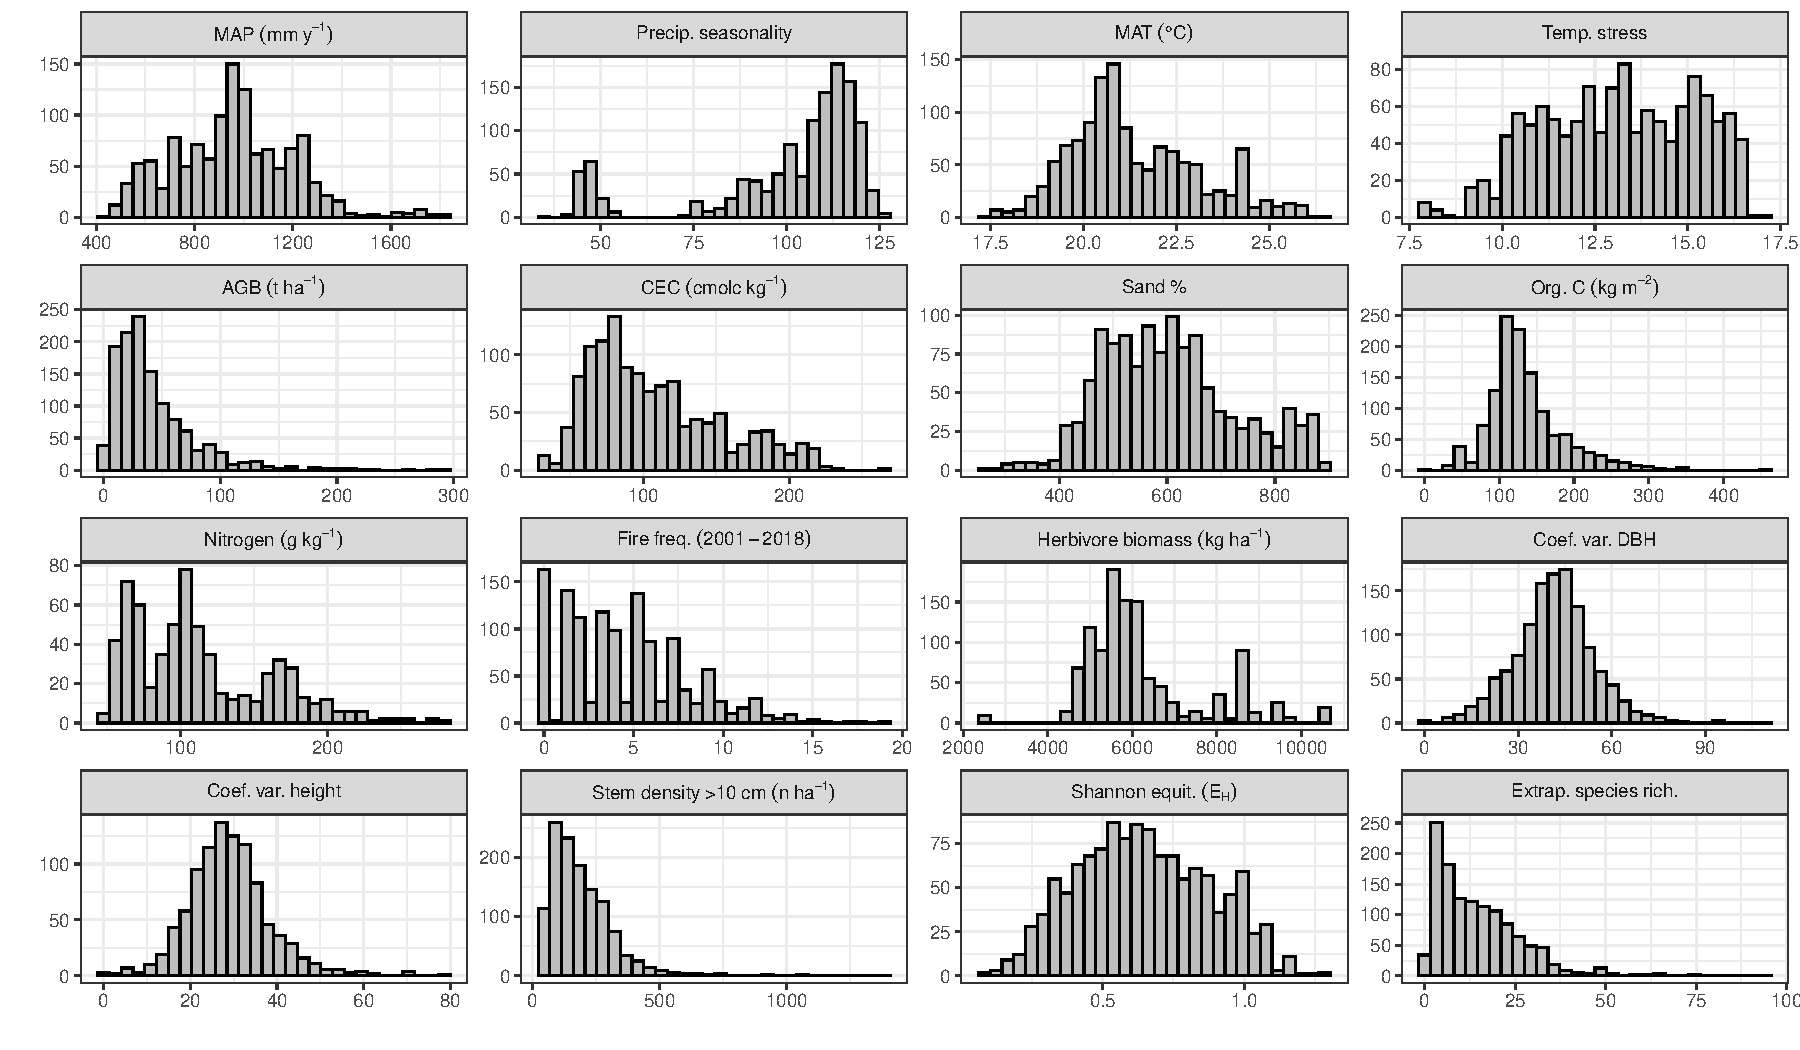
\includegraphics[width=\linewidth]{img/hist_raw}
	\caption[Raw histograms of observed variables]{Histograms of raw untransformed observed variables used in final analyses.}
	\label{befr:hist_raw}
\end{figure}

\begin{figure}[H]
	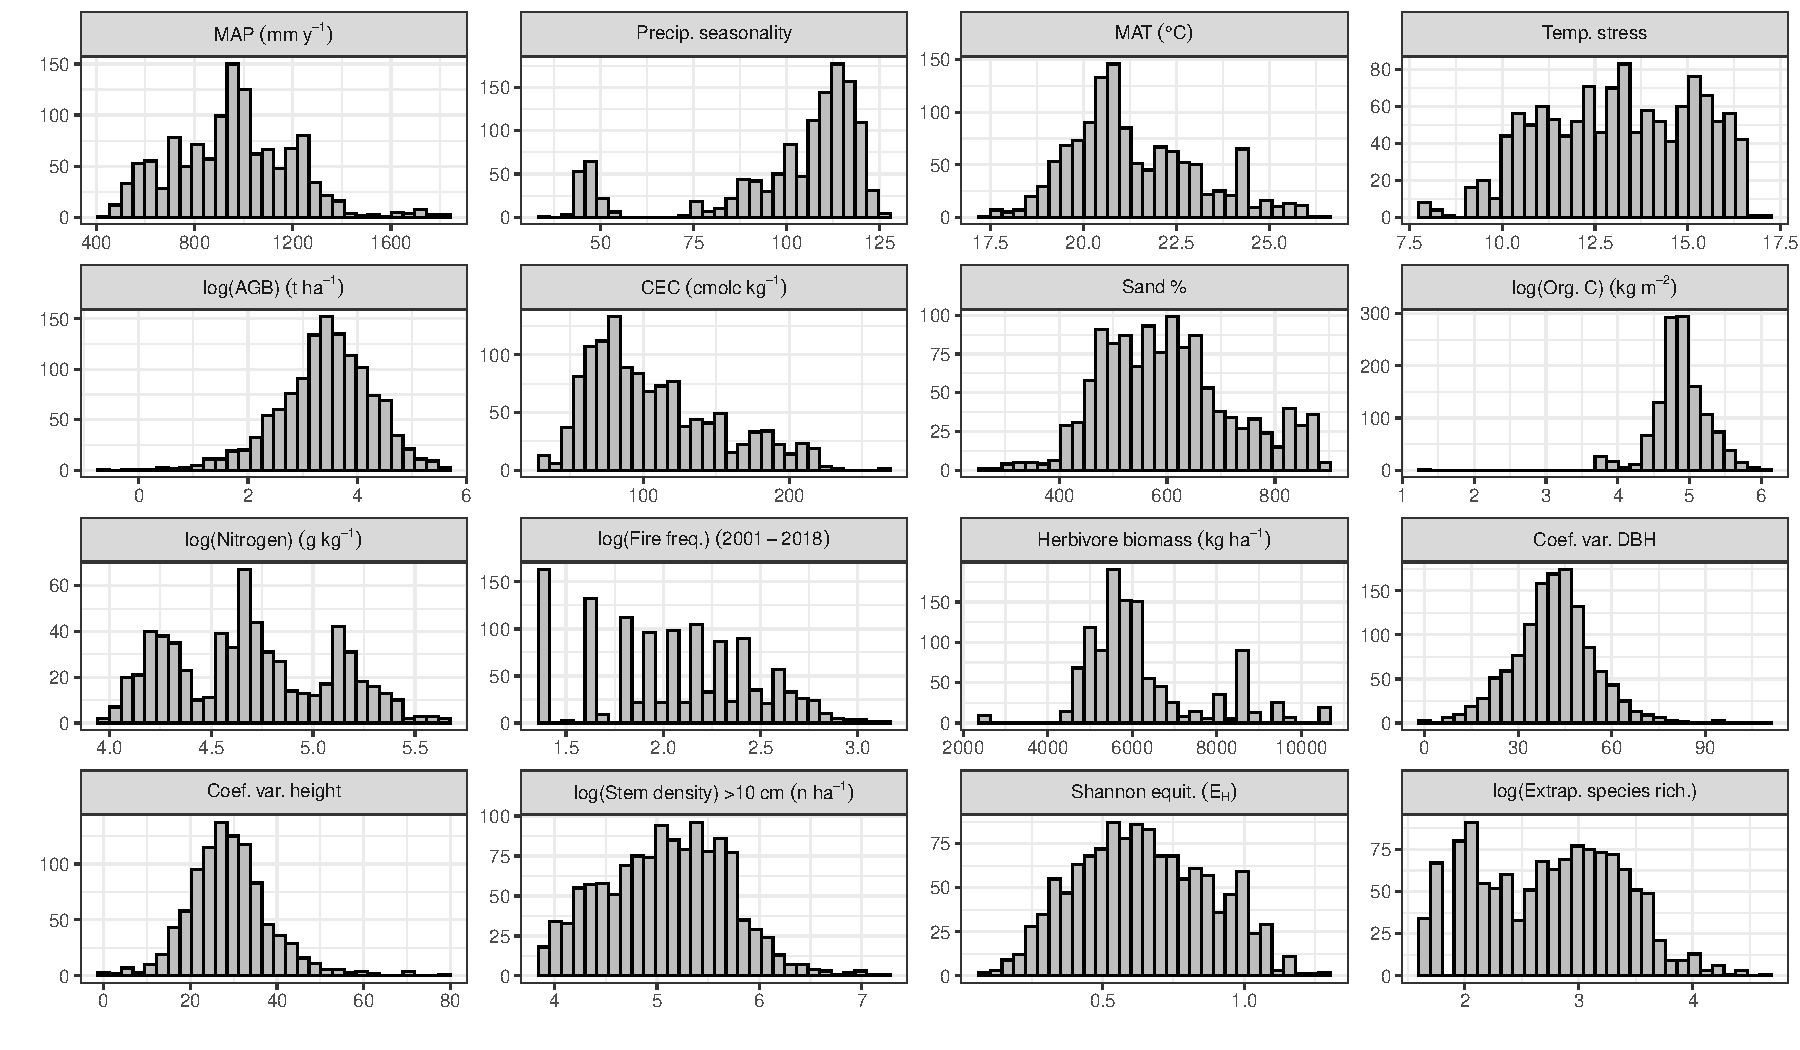
\includegraphics[width=\linewidth]{img/hist_trans}
	\caption[Histograms of transformed observed variables]{Histograms of observed variables transformed to achieve a normal frequency distribution.}
	\label{befr:hist_trans}
\end{figure}

\begin{longtable}[H]{llS[table-format=-1.2]S[table-format=-1.2]S[table-format=-1.2]S[table-format=4.0]S[table-format=<1.2]}
\caption[Correlation fit statistics]{Correlation fit statistics among observed variables used in path analysis. Showing the Pearson correlation coefficient ($r$), correlation confidence interval upper and lower bounds, number of plots used in the correlation (n), and the p-value of the correlation (Prob.).} 
\label{befr:corr_ci} \\
\toprule
{X} & {Y} & {$r$} & {Lower} & {Upper} & {N} & {Prob.} \\ 
\midrule
\endfirsthead
\toprule
{X} & {Y} & {$r$} & {Lower} & {Upper} & {N} & {Prob.} \\ 
\midrule
\endhead
Soil CEC & Soil C & 0.26 & 0.21 & 0.31 & 1239 & <0.01 \\ 
Soil N & Soil C & 0.85 & 0.82 & 0.87 & 644 & <0.01 \\ 
Fire freq. & Soil C & -0.07 & -0.13 & -0.01 & 1239 & <0.05 \\ 
MAP & Soil C & 0.51 & 0.46 & 0.55 & 1239 & <0.01 \\ 
Precip. seas. & Soil C & -0.56 & -0.60 & -0.52 & 1239 & <0.01 \\ 
Temp. stress & Soil C & -0.63 & -0.67 & -0.60 & 1239 & <0.01 \\ 
Sand \% & Soil C & -0.57 & -0.61 & -0.54 & 1239 & <0.01 \\ 
Species rich. & Soil C & 0.25 & 0.20 & 0.30 & 1239 & <0.01 \\ 
Shannon equit. & Soil C & 0.23 & 0.18 & 0.28 & 1239 & <0.01 \\ 
Height CV & Soil C & 0.23 & 0.17 & 0.29 & 981 & <0.01 \\ 
DBH CV & Soil C & 0.16 & 0.11 & 0.22 & 1237 & <0.01 \\ 
Stem density & Soil C & 0.07 & 0.02 & 0.13 & 1239 & <0.05 \\ 
AGB & Soil C & 0.26 & 0.21 & 0.32 & 1239 & <0.01 \\ 
Soil N & Soil CEC & 0.44 & 0.37 & 0.50 & 644 & <0.01 \\ 
Fire freq. & Soil CEC & -0.47 & -0.51 & -0.43 & 1239 & <0.01 \\ 
MAP & Soil CEC & -0.28 & -0.33 & -0.22 & 1239 & <0.01 \\ 
Precip. seas. & Soil CEC & -0.71 & -0.73 & -0.68 & 1239 & <0.01 \\ 
Temp. stress & Soil CEC & -0.25 & -0.30 & -0.20 & 1239 & <0.01 \\ 
Sand \% & Soil CEC & -0.21 & -0.27 & -0.16 & 1239 & <0.01 \\ 
Species rich. & Soil CEC & -0.38 & -0.43 & -0.33 & 1239 & <0.01 \\ 
Shannon equit. & Soil CEC & -0.09 & -0.15 & -0.04 & 1239 & <0.01 \\ 
Height CV & Soil CEC & -0.11 & -0.17 & -0.05 & 981 & <0.01 \\ 
DBH CV & Soil CEC & -0.01 & -0.07 & 0.04 & 1237 & 0.62 \\ 
Stem density & Soil CEC & -0.02 & -0.08 & 0.03 & 1239 & 0.43 \\ 
AGB & Soil CEC & -0.04 & -0.09 & 0.02 & 1239 & 0.17 \\ 
Fire freq. & Soil N & -0.25 & -0.32 & -0.18 & 644 & <0.01 \\ 
MAP & Soil N & 0.37 & 0.30 & 0.44 & 644 & <0.01 \\ 
Precip. seas. & Soil N & -0.76 & -0.79 & -0.73 & 644 & <0.01 \\ 
Temp. stress & Soil N & -0.80 & -0.82 & -0.77 & 644 & <0.01 \\ 
Sand \% & Soil N & -0.66 & -0.70 & -0.61 & 644 & <0.01 \\ 
Species rich. & Soil N & 0.44 & 0.38 & 0.50 & 644 & <0.01 \\ 
Shannon equit. & Soil N & 0.35 & 0.28 & 0.42 & 644 & <0.01 \\ 
Height CV & Soil N & 0.27 & 0.18 & 0.36 & 386 & <0.01 \\ 
DBH CV & Soil N & 0.26 & 0.18 & 0.33 & 642 & <0.01 \\ 
Stem density & Soil N & -0.03 & -0.11 & 0.05 & 644 & 0.47 \\ 
AGB & Soil N & 0.31 & 0.24 & 0.38 & 644 & <0.01 \\ 
MAP & Fire freq. & 0.37 & 0.32 & 0.42 & 1239 & <0.01 \\ 
Precip. seas. & Fire freq. & 0.36 & 0.31 & 0.41 & 1239 & <0.01 \\ 
Temp. stress & Fire freq. & 0.21 & 0.16 & 0.26 & 1239 & <0.01 \\ 
Sand \% & Fire freq. & 0.06 & 0.00 & 0.11 & 1239 & <0.05 \\ 
Species rich. & Fire freq. & 0.38 & 0.34 & 0.43 & 1239 & <0.01 \\ 
Shannon equit. & Fire freq. & 0.12 & 0.07 & 0.18 & 1239 & <0.01 \\ 
Height CV & Fire freq. & 0.15 & 0.09 & 0.22 & 981 & <0.01 \\ 
DBH CV & Fire freq. & 0.12 & 0.07 & 0.18 & 1237 & <0.01 \\ 
Stem density & Fire freq. & -0.02 & -0.07 & 0.04 & 1239 & 0.52 \\ 
AGB & Fire freq. & 0.03 & -0.03 & 0.08 & 1239 & 0.33 \\ 
Precip. seas. & MAP & -0.07 & -0.12 & -0.01 & 1239 & <0.05 \\ 
Temp. stress & MAP & -0.49 & -0.53 & -0.44 & 1239 & <0.01 \\ 
Sand \% & MAP & -0.33 & -0.38 & -0.28 & 1239 & <0.01 \\ 
Species rich. & MAP & 0.41 & 0.36 & 0.45 & 1239 & <0.01 \\ 
Shannon equit. & MAP & 0.15 & 0.10 & 0.20 & 1239 & <0.01 \\ 
Height CV & MAP & 0.25 & 0.19 & 0.30 & 981 & <0.01 \\ 
DBH CV & MAP & 0.11 & 0.06 & 0.17 & 1237 & <0.01 \\ 
Stem density & MAP & 0.02 & -0.03 & 0.08 & 1239 & 0.47 \\ 
AGB & MAP & 0.24 & 0.18 & 0.29 & 1239 & <0.01 \\ 
Temp. stress & Precip. seas. & 0.50 & 0.45 & 0.54 & 1239 & <0.01 \\ 
Sand \% & Precip. seas. & 0.31 & 0.26 & 0.36 & 1239 & <0.01 \\ 
Species rich. & Precip. seas. & 0.12 & 0.07 & 0.18 & 1239 & <0.01 \\ 
Shannon equit. & Precip. seas. & -0.07 & -0.12 & -0.01 & 1239 & <0.05 \\ 
Height CV & Precip. seas. & -0.05 & -0.11 & 0.01 & 981 & 0.11 \\ 
DBH CV & Precip. seas. & -0.10 & -0.15 & -0.04 & 1237 & <0.01 \\ 
Stem density & Precip. seas. & -0.04 & -0.10 & 0.01 & 1239 & 0.12 \\ 
AGB & Precip. seas. & -0.18 & -0.23 & -0.13 & 1239 & <0.01 \\ 
Sand \% & Temp. stress & 0.30 & 0.25 & 0.35 & 1239 & <0.01 \\ 
Species rich. & Temp. stress & -0.13 & -0.18 & -0.07 & 1239 & <0.01 \\ 
Shannon equit. & Temp. stress & -0.13 & -0.18 & -0.07 & 1239 & <0.01 \\ 
Height CV & Temp. stress & -0.14 & -0.20 & -0.08 & 981 & <0.01 \\ 
DBH CV & Temp. stress & -0.04 & -0.10 & 0.01 & 1237 & 0.12 \\ 
Stem density & Temp. stress & 0.03 & -0.02 & 0.09 & 1239 & 0.27 \\ 
AGB & Temp. stress & -0.17 & -0.22 & -0.11 & 1239 & <0.01 \\ 
Species rich. & Sand \% & -0.27 & -0.32 & -0.22 & 1239 & <0.01 \\ 
Shannon equit. & Sand \% & -0.21 & -0.26 & -0.16 & 1239 & <0.01 \\ 
Height CV & Sand \% & -0.24 & -0.30 & -0.18 & 981 & <0.01 \\ 
DBH CV & Sand \% & -0.16 & -0.21 & -0.10 & 1237 & <0.01 \\ 
Stem density & Sand \% & -0.14 & -0.19 & -0.08 & 1239 & <0.01 \\ 
AGB & Sand \% & -0.22 & -0.27 & -0.16 & 1239 & <0.01 \\ 
Shannon equit. & Species rich. & 0.60 & 0.56 & 0.63 & 1249 & <0.01 \\ 
Height CV & Species rich. & 0.31 & 0.25 & 0.36 & 981 & <0.01 \\ 
DBH CV & Species rich. & 0.32 & 0.26 & 0.36 & 1247 & <0.01 \\ 
Stem density & Species rich. & 0.23 & 0.17 & 0.28 & 1249 & <0.01 \\ 
AGB & Species rich. & 0.33 & 0.28 & 0.38 & 1249 & <0.01 \\ 
Height CV & Shannon equit. & 0.14 & 0.07 & 0.20 & 981 & <0.01 \\ 
DBH CV & Shannon equit. & 0.23 & 0.17 & 0.28 & 1247 & <0.01 \\ 
Stem density & Shannon equit. & 0.41 & 0.36 & 0.45 & 1249 & <0.01 \\ 
AGB & Shannon equit. & 0.38 & 0.33 & 0.42 & 1249 & <0.01 \\ 
DBH CV & Height CV & 0.49 & 0.44 & 0.54 & 981 & <0.01 \\ 
Stem density & Height CV & 0.00 & -0.06 & 0.06 & 981 & 0.95 \\ 
AGB & Height CV & 0.24 & 0.18 & 0.30 & 981 & <0.01 \\ 
Stem density & DBH CV & 0.11 & 0.05 & 0.16 & 1247 & <0.01 \\ 
AGB & DBH CV & 0.44 & 0.40 & 0.49 & 1247 & <0.01 \\ 
AGB & Stem density & 0.57 & 0.53 & 0.61 & 1249 & <0.01 \\ 
\bottomrule
\end{longtable}


\begin{figure}[H]
	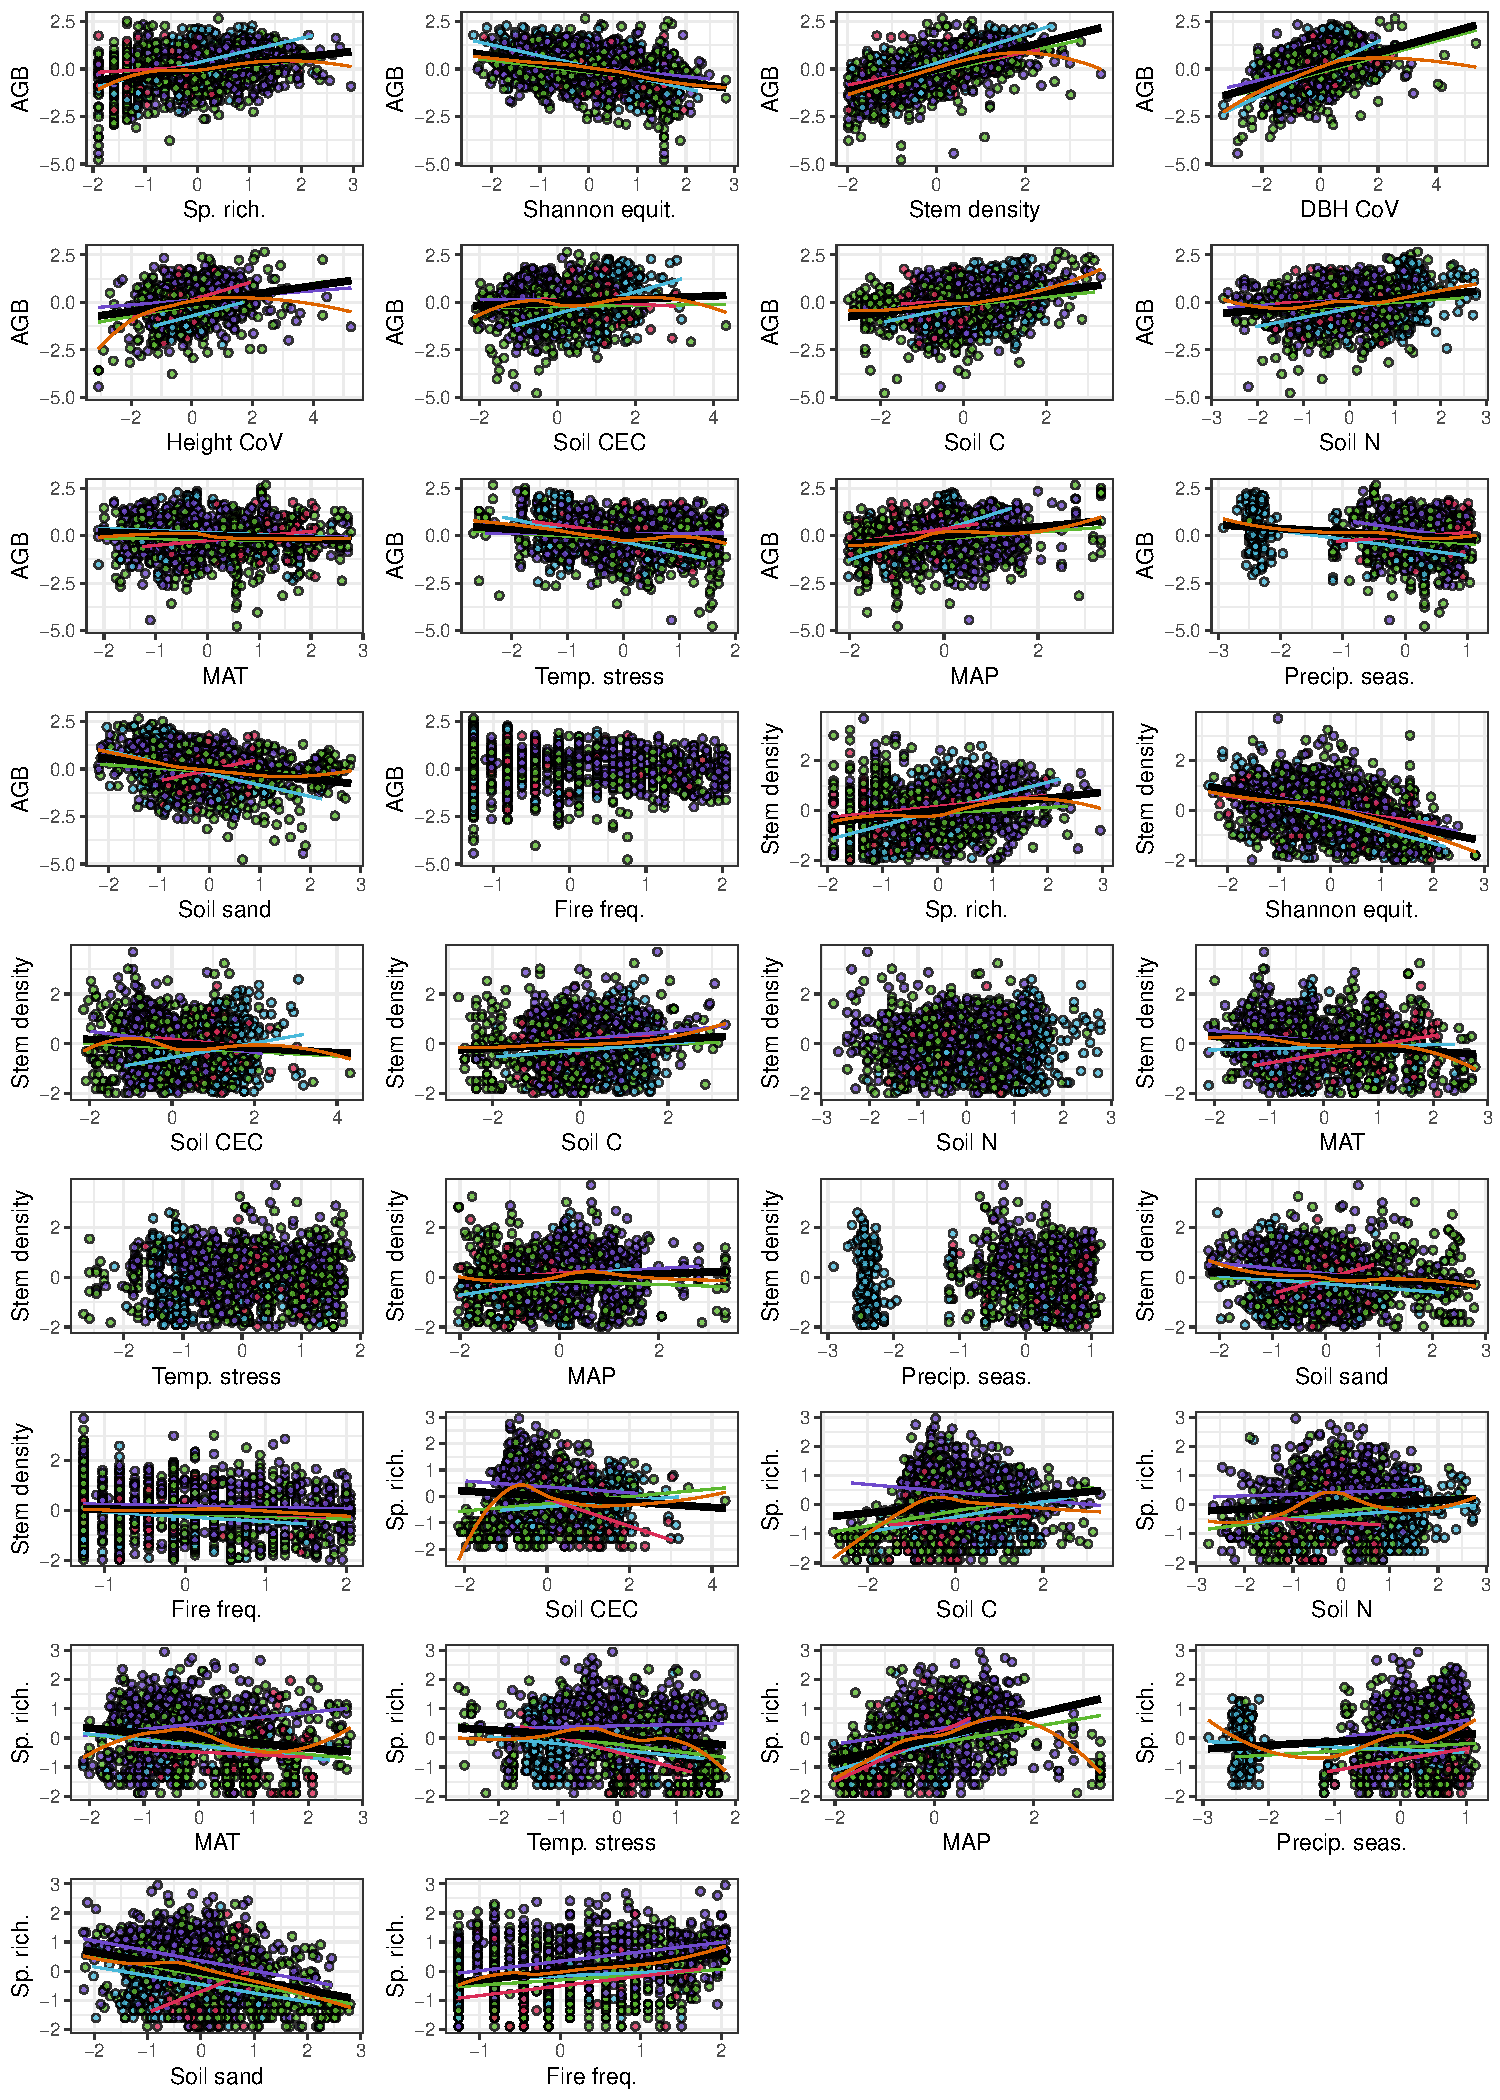
\includegraphics[width=0.9\linewidth]{img/bivar_lm}
	\caption[Bivariate scatter plots of observed variables]{\setstretch{1}Bivariate scatter plots for each observed variable used in the SEMs (Structural Equation Models), based on hypothesised paths of causality. Points are coloured according to vegetation type: green = Baikiaea, purple = Core miombo, blue = ex-Acacia, red = Mopane. The black line combines all vegetation types in a single linear regression, while loess trend lines are fitted for each vegetation type, separately. An orange loess trend line is fitted for all the data. All data is standardised to a mean of zero and a standard deviation of one. Variables are transformed where it was appropriate for analysis.}
	\label{befr:bivar_lm}
\end{figure}

\begin{figure}[H]
	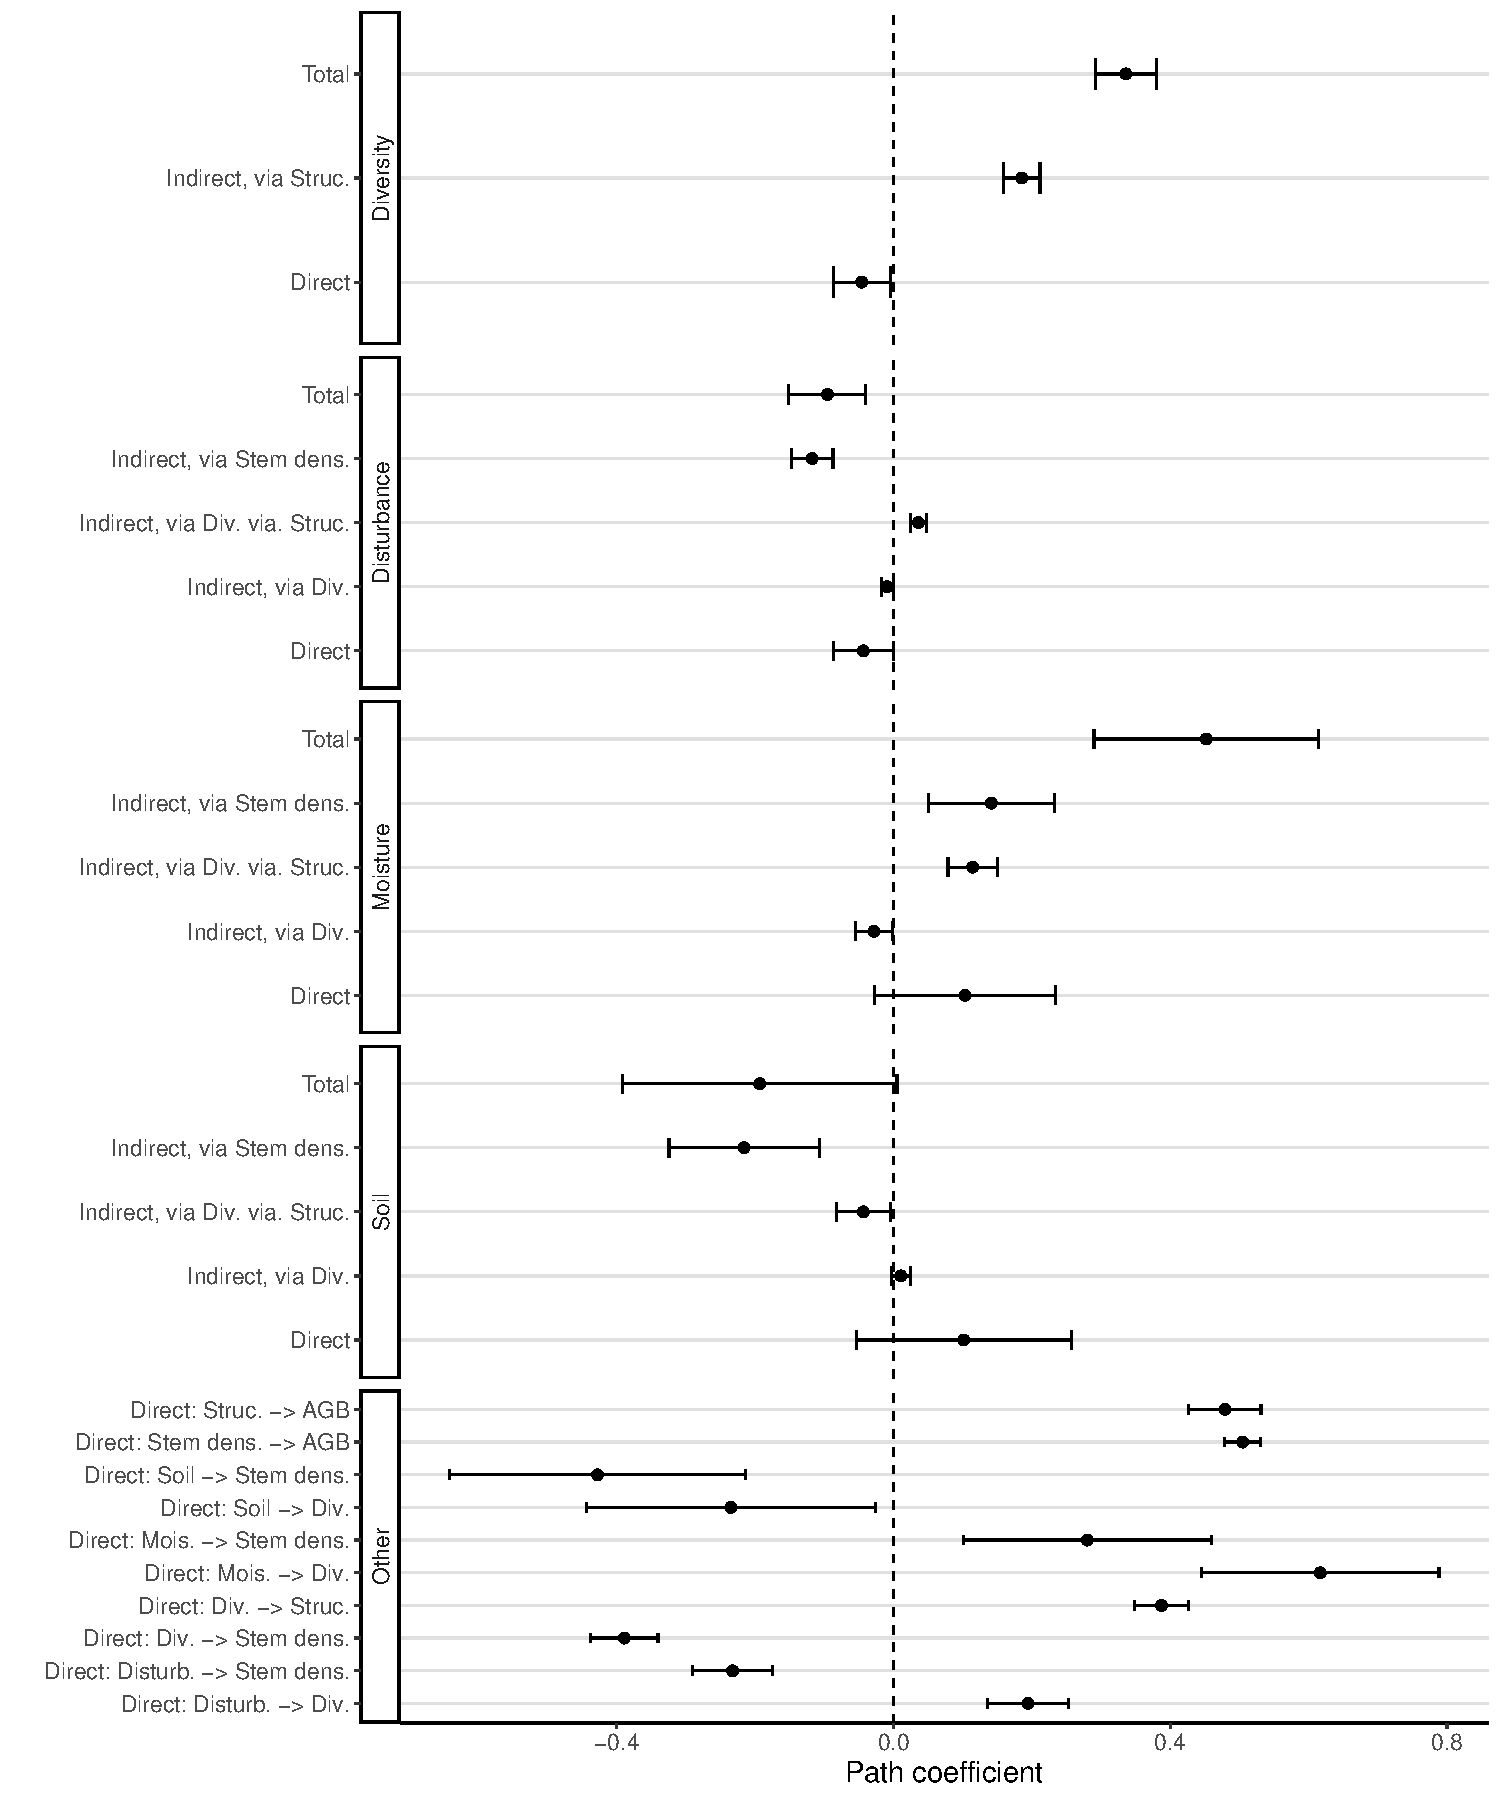
\includegraphics[width=\linewidth]{img/full_model_slopes}
	\caption[Path coefficients for full Structural Equation Model]{Unstandardised path coefficients for the full model including tree species diversity, environmental covariates and stem density. Path coefficients are $\pm1$ standard error. Path coefficients where the interval (standard error) does not overlap zero are considered to be significant effects.}
	\label{befr:full_model_slopes}
\end{figure}

\end{supplement}

\end{refsection}

